\documentclass[12pt]{article}

\usepackage{sbc-template}
\usepackage{verbatim}
\setcounter{secnumdepth}{4}
\usepackage{graphicx,url}

\usepackage{amsfonts}
\usepackage{amsmath}
\usepackage{multicol}

\usepackage[brazil]{babel}   
%\usepackage[latin1]{inputenc}  
\usepackage[utf8]{inputenc}  
% UTF-8 encoding is recommended by ShareLaTex

%==========================================================
% ToDo notes
%==========================================================
\usepackage{todonotes}
\usepackage{xargs}                      % Use more than one optional parameter in a new commands
%\usepackage[disable]{todonotes}   % uncomment for final version
% \presetkeys{todonotes}{inline}{}  %% Make todo notes inline by default.
\newcommandx{\todobase}[3][2=noinline]{\todo[fancyline,linecolor=#1,backgroundcolor=#1!25,bordercolor=#1,#2]{#3}}
%\newcommand{\myreminder}[1]{\todo[inline,linecolor=cyan,backgroundcolor=cyan!25,bordercolor=cyan]{#1}}
%\newcommand{\NSLDS}[1]{\todo[inline,linecolor=cyan,backgroundcolor=cyan!25,bordercolor=cyan]{#1}}
\newcommandx{\thiswillnotshow}[2][1=]{\todo[fancyline,disable,#1]{#2}}
\newcommandx{\erick}[2][1=]{\todobase{yellow}[#1]{#2}}
\newcommandx{\lucas}[2][1=]{\todobase{green}[#1]{#2}}
\newcommandx{\ricardo}[2][1=]{\todobase{blue}[#1]{#2}}

%==========================================================
% Finite Field
%==========================================================
\newcommand{\Fp}{$\mathbb{F}_p$}
\newcommand{\Fpfull}{$\mathbb{F}_{2^{255}-19}$}
%\ceil and \floor
\usepackage{mathtools}
\DeclarePairedDelimiter\ceil{\lceil}{\rceil}
\DeclarePairedDelimiter\floor{\lfloor}{\rfloor}
% alias for assignment arrow
\newcommand{\rcv}{\leftarrow}

%==========================================================
% Algorithms
%==========================================================
\usepackage{algorithm}
\usepackage{algorithmic}
\renewcommand{\algorithmicrequire} {\textbf{\textsc{Inputs:}}}
\renewcommand{\algorithmicensure}  {\textbf{\textsc{Outputs:}}}
\usepackage{enumitem}

%===============================================================
% Package to simplify referencing of section, figure, algorithm, etc.
% Must be loaded AFTER hyperref.
%===============================================================
\usepackage{cleveref}

%===========================================================
% Global constants for table formatting settings
\newcommand{\tblvertpaddingfactor}{1.3}
\newcommand{\tblhorizpadding}{3pt}
%===========================================================

\sloppy

%\title{Canais laterais em criptografia simétrica e de curvas elípticas: ataques e contramedidas\footnote{Esse trabalho é uma versão aprofundada e modernizada do minicurso ministrado no SBSeg 2009 por João Paulo Fernandes Ventura e Ricardo Dahab}}

\title{Canais laterais em criptografia simétrica e de curvas elípticas: ataques e contramedidas}

\author{Lucas Zanco Ladeira\inst{1} (apresentador), Erick Nascimento\inst{1}, \\ Ricardo Dahab\inst{1}, Diego Aranha\inst{1}, Julio Lopez\inst{1}}


\address{Instituto de Computação – Universidade Estadual de Campinas (Unicamp)\\
Caixa Postal 6176 – 13.084-970 – Campinas – SP – Brasil
    \email{lucas.ladeira@students.ic.unicamp.br}
  \email{erick.nogueira.nascimento@gmail.com}
  \email{\{rdahab,dfaranha,jlopez\}@ic.unicamp.br}
}

\begin{document} 

\maketitle
     
\begin{resumo}
Existe uma infinidade de ataques visando a quebra de sistemas criptogr\'aficos, buscando a obtenção de informação sigilosa, acesso não-autorizado, entre outros. Tais ataques ocorrem tanto sobre os algoritmos quanto implementações de um sistema. Um tipo de ataque sobre implementações \'e o de canais laterais, que faz uso do vazamento de informa\c{c}\~oes durante a execu\c{c}\~ao de alguma primitiva criptogr\'afica. Ataques dessa categoria utilizam variações do tempo de execução, do consumo de pot\^encia, do campo magn\'etico, entre outros. As contramedidas podem ser baseadas em modificações no software ou no hardware. Neste minicurso, nossa atenção se restringe ao software, voltada para métodos criptográficos simétricos, e os assimétricos baseados em curvas elípticas.
\end{resumo}



\section{Introdução}

\section{Encriptação simétrica e hash}



\pagebreak
\section{Criptografia de curvas elípticas (ECC)}
Criptografia de curvas elípticas é uma classe de algoritmos criptográficos que se baseia na aritmética de pontos de uma curva elíptica em um corpo finito $\mathbb{F}$ \cite{Hankerson:2003:GEC:940321}. Os algoritmos criptográficos que utilizam esse tipo de problema matemático podem se diferenciar de acordo com vários fatores, como por exemplo: o primo utilizado, a curva, corpo finito $\mathbb{F}_p$ ou $\mathbb{F}_{2^m}$, o mapeamento dos pontos na curva, entre outros. 

As operações mais simples executadas em uma curva é a adição de pontos e a duplicação de um ponto, sendo $R = P + Q$ e $R = P + P$ respectivamente. Dependendo da curva utilizada é possível executar essas operações de maneira mais eficiente podendo diferenciar o mapeamento desses pontos na curva.

Seguindo a notação descrita por \cite{Hankerson:2003:GEC:940321} podemos definir uma curva elíptica $E$ como: $E: y^2 + a_1xy + a_3y = x^3 + a_2x^2 + a_4x + a_6$ sobre um corpo K. Onde $\bigtriangleup \neq 0$, essa condição garante que não existirá ponto onde a curva possui duas ou mais linhas de tangente diferentes. A linha da tangente é utilizada na operação de duplicação de um ponto. Sendo que, $\bigtriangleup$ é definido como:

\begin{align*}
\bigtriangleup &= -d_2^2d_8 - 8d_4^3 - 27d_6^2 + 9d_2d_4d_6 \\
d_2 &= a_1^2 + 4a_2 \\
d_4 &= 2a_4 + a_1a_3 \\ 
d_6 &= a_3^2 + 4a_6 \\
d_8 &= a_1^2a_6 + 4a_2a_6 - a_1a_3a_4 + a_2a_3^2 - a_4^2
\end{align*}

A curva descrita anteriormente é chamada de equação de Weiertrass, onde a mesma possui uma forma simplificada: $y^2 = x^3 + ax + b$. Essa equação é utilizada como ponto inicial para descrição de várias curvas, sendo que pode-se variar os valores de $a$ e $b$ para obter diferentes curvas. Durante a escolha de qual utilizar é possível verificar a facilidade de implementação, possibilidade de paralelização, e também o desempenho da mesma. 

O desempenho está ligado as operações executadas, como por exemplo o método Montgomery-Ladder utilizado durante a multiplicação escalar, e pelas instruções do processador que facilitam a aritmética. Na seção a seguir iremos exibir as curvas com mais ocorrência na literatura, e algumas propriedades de cada uma.

\subsection{Curvas NIST e curvas modernas}
Primeiramente iremos apresentar as curvas NIST, essas curvas são recomendações de utilização feitas pelo NIST (National Institute of Standards and Technlogy), situado nos Estados Unidos da América. As mesmas foram geradas de forma pseudo-aleatória pela NSA, e possuem ao todo são 10 corpos finitos sendo 5 corpos primos ($\mathbb{F}_p$) e 5 corpos binários ($\mathbb{F}_{2^m}$) \cite{Brown2001}.

Os corpos foram recomendados com o foco no desempenho das curvas, facilitando a aritmética utilizada. Todavia existe uma resistência da comunidade em adotar o que foi proposto, pela incerteza na existência de vulnerabilidades, inseridas para obter informações secretas pelo governo norte americano. Os corpos finitos recomendados podem ser observados a seguir, sendo P os corpos primos e B as corpos binários:

\begin{multicols}{2}
\begin{itemize}
\item P-192 \\ $\mathbb{F}_{192}$ $p = 2^{192} - 2^{64} - 1$; 
\item P-224 \\ $\mathbb{F}_{224}$ $p = 2^{224} - 2^{96} + 1$;
\item P-256 \\ $\mathbb{F}_{256}$ $p = 2^{256} - 2^{224} + 2^{192} + 2^{96} - 1$;
\item P-384 \\ $\mathbb{F}_{384}$ $p = 2^{384} - 2^{128} - 2^{96} + 2^{32} - 1$;
\item P-521 \\ $\mathbb{F}_{521}$ $p = 2^{521} - 1$;
\item B-163 \\ $\mathbb{F}_{2^{163}}$ $f(x) = x^{163} + x^7 + x^6 + x^3 + 1$;
\item B-233 \\ $\mathbb{F}_{2^{233}}$ $f(x) = x^{233} + x^{74} + 1$;
\item B-283 \\ $\mathbb{F}_{2^{283}}$ $f(x) = x^{283} + x^{12} + x^7 + x^5 + 1$;
\item B-409 \\ $\mathbb{F}_{2^{409}}$ $f(x) = x^{409} + x ^{87} + 1$;
\item B-571 \\ $\mathbb{F}_{2^{571}}$ $f(x) = x^{571} + x^{10} + x^5 + x^2 + 1$.
\end{itemize}
\end{multicols}

Nesses corpos finitos primos é recomendado utilizar as curvas pseudo-aleatórias, já no caso dos corpos binários recomenda-se, além da utilização das curvas pseudo-aleatórias, o uso da curva de Koblitz. A geração de curvas pseudo-aleatórias segue três passos: primeiramente é gerada uma semente, após a partir da semente é gerada uma curva. Por fim, é verificado se a curva gerada é resistente aos ataques conhecidos, caso não seja o processo é repetido.

Existem duas curvas elípticas que estão se destacando considerando o desempenho obtido junto à técnicas de multiplicação escalar eficiente, redução modular, entre outras. Elas são a curva de Montgomery e a curva de Edwards, onde é possível encontrar implementações resistentes a ataques de canal lateral como ataque por tempo e ataque por cache.

A curva de Montgomery tem a seguinte equação: $E: y^2 = x^3 + Ax^2 + x$. O valor do parâmetro $A$ pode ser alterado para melhorar o desempenho das multiplicações escalares. Iremos tratar a utilização dessa curva com o primo $25519$ $(2^{255}-19)$ e o valor de $A = 486662$, dessa maneira a curva é definida sobre o corpo $\mathbb{F}_{2^{255}-19}$ \cite{Dull:2015:HCM:2834659.2834708}. Considerando o corpo finito utilizado essa curva é chamada de 25519, onde os pontos na curva são mapeados como $P = (X : Z)$. 

A curva de Edwards tem a fórmula: $E: -x^2 + y^2 = 1 + dx^2y^2$ \cite{Bernstein2012}. Nessa curva a soma de dois pontos segue a \textit{Edwards addition law}:
$$ (x_1,y_1) + (x_2,y_2) = (\frac{x_1y_2 + x_2y_1}{1 + xd_1x_2y_1y_2},\frac{y_1y_2 + x_1x_2}{1 - dx_1x_2y_1y_2}) $$
Já a duplicação de um ponto segue a mesma fórmula da adição, portanto a diferença é que ambos os pontos possuem os mesmos valores, sendo: $(x_1, y_1) + (x_1, y_1)$.

\subsection{Algoritmos para multiplicação escalar (ECSM) básicos}
Considerando que a principal operação em curvas elípticas é a multiplicação escalar é necessário explorar as diferentes formas de implementar esse calculo. Nessa seção serão apresentados os mais simples, resistentes ou não a ataques de canal lateral, e pequenas variações criando novos algoritmos com propriedades diferentes.

O primeiro é o método \textit{Double-and-add} (também conhecido como \textit{Double-and-add-not-always}), o mesmo é utilizado para calcular $dP$. Ele possui quatro variáveis, sendo $N$ para armazenar o resultado da operação de duplicação do ponto durante a execução, $Q$ armazena o resultado das operações, $P$ é o ponto escolhido na curva para a multiplicação escalar, e por fim $k$ é a chave utilizada na multiplicação.

É importante citar que $m$ é o tamanho da chave em bits, sendo que cada \textit{bit} da chave será utilizado nesse método, totalizando 256 execuções para uma chave de 32 \textit{bytes}. O algoritmo 1 é chamado também de \textit{left-to-right} considerando a orientação onde são percorridos os \textit{bits} da chave privada. É necessário citar que esse algoritmo não é resistente a ataques de canal lateral, sendo que existe uma variação de tempo dependendo do valor dos bits da chave.

\floatname{algorithm}{Algoritmo}
\begin{algorithm}[H]
\caption{Double-and-add left-to-right}
\begin{algorithmic} 
    \REQUIRE $P, k$
    \ENSURE $Q = kP$
    \STATE $N \leftarrow P$
    \STATE $Q \leftarrow 0$
    \FOR{$i$ from $m-1$ \TO $0$} 
        \STATE $N \leftarrow 2N$
        \IF{$k_i = 1$}
            \STATE $Q \leftarrow Q+N$
        \ENDIF
    \ENDFOR
    \RETURN Q
    \end{algorithmic}
\end{algorithm}

Uma outra maneira de percorrer os \textit{bits} de \textit{d} é do \textit{bit} menos significativo para o  mais significativo, e é conhecida como \textit{right-to-left}. A mesma apresenta pequenas diferenças em relação ao algoritmo 1 em termos do código, modificando apenas a ordem dos \textit{bits} percorridos e a ordem as operações de adição e duplicação. Já em relação à segurança esse também não é resistente a ataques de canal lateral.

\floatname{algorithm}{Algoritmo}
\begin{algorithm}[H]
\caption{Double-and-add right-to-left}
\begin{algorithmic} 
    \REQUIRE $P, k$
    \ENSURE $Q = kP$
    \STATE $N \leftarrow P$
    \STATE $Q \leftarrow 0$
    \FOR{$i$ from $0$ \TO $m$} 
        \IF{$k_i = 1$}
            \STATE $Q \leftarrow Q + N$
        \ENDIF
        \STATE $N \leftarrow 2N$
    \ENDFOR
    \RETURN Q
    \end{algorithmic}
\end{algorithm}

Na seção 3.4 iremos tratar outros método de multiplicação escalar que são resistentes a ataques de canal lateral, tornando constante o número de operações executadas em cada iteração e o tempo de execução independente do valor da chave.

\subsection{Uso de tabelas precomputadas para melhorar desempenho; algoritmos de janela fixa}
Considerando a utilização de um ponto $P$ fixo, é possível executar o pré-processamento da exponenciação de $P$ e armazenar em uma tabela para ser utilizada em várias multiplicações escalares diferentes. Consequentemente existe um ganho de desempenho em relação a mesma implementação sem a utilização da tabela, pois torna rápida a multiplicação escalar onde a fatoração de $P$ é utilizada. Isso é possível considerando que o maior custo do algoritmo é na geração da tabela, tornando eficiente a partir da primeira multiplicação escalar.

Um exemplo disso é um ponto $P$ fixo, os seguintes valores são pré-computados: $2P, 2^2P, 2^3P,..., 2^mP$, sendo $m$ a quantidade de bits do multiplicador escalar $k$. Dessa maneira qualquer operação de duplicação do ponto já foi calculada. Agora iremos apresentar um algoritmo que faz esse pré-processamento que foi proposto por Brickell, Gordon, McCurley, e Wilson. 

\subsection{Algoritmos regulares; atomicidade; montgomery ladder}
Para que algoritmos de multiplicação escalar sejam resistentes à ataques de canal lateral é necessário que o fluxo de execução seja regular, isso significa que as operações a serem executadas não serão alteradas de acordo com o valor da chave privada. É possível observar que com essas alterações o tempo de execução será constante, já se tornando resistência minimamente ao ataque de canal lateral de tempo.

Primeiramente iremos apresentar o algoritmo chamado \textit{Double-and-add-always}, proposto por Coron, onde o mesmo executa a adição e duplicação do ponto em todas a iterações. O pseudo-código pode ser observado no algoirtmo 3. Da mesma maneira dos outros algoritmos de multiplicação escalar apresentados os parâmetros de entrada são o ponto $P$ e o escalar $k$, e a saída é o resultado da computação $Q$.

\begin{algorithm}[H]
\caption{Double-and-add-always}
\begin{algorithmic} 
    \REQUIRE $P, k$
    \ENSURE $Q = kP$
    \STATE $R_0 \leftarrow P$
    \FOR{$i$ from $m-2$ \TO $0$} 
        \STATE $R_0 \leftarrow 2R_0$
        \STATE $R_1 \leftarrow R_0 + P$
        \STATE $b \leftarrow k_{i}$
        \STATE $R_0 \leftarrow R_b$
    \ENDFOR
    \RETURN $R_0$
    \end{algorithmic}
\end{algorithm}

Uma implementação mais promissora que a apresentada anteriormente é chamada de \textit{Atomic Double-and-Add}. Na mesma não é possível diferenciar qual operação no ponto está sendo executada. Além disso, no algoritmo o ponto principal da segurança está na execução da operação de $\oplus$ entre $b$ e os \textit{bits} da chave, sendo que a operação de $\oplus$ não vaza informações sobre a chave. O pseudocódigo do algoritmo pode ser observado no algoritmo 4, tendo entradas o ponto $P$ e o escalar $k$.

\begin{algorithm}[H]
\caption{Atomic Double-and-Add}
\begin{algorithmic} 
    \REQUIRE $P, k$
    \ENSURE $Q = kP$
    \STATE $R_0 \leftarrow P$
    \STATE $R_1 \leftarrow P$
    \STATE $j \leftarrow l - 2$
    \STATE $b \leftarrow 0$
    \WHILE{$j \ge 0$} 
        \STATE $R_0 \leftarrow R_0 + R_b$
        \STATE $b \leftarrow b \oplus k_j$
        \STATE $j \leftarrow j + k_j -1$
    \ENDWHILE
    \RETURN $R_0$
    \end{algorithmic}
\end{algorithm}


Um outro algoritmo que iremos apresentar é chamado de \textit{Montgomery Ladder}, o mesmo apresenta eficiência na multiplicar escalar em comparação com os outros e possui vantagens dependendo da curva e do primo utilizado no esquema criptográfico. Primeiramente iremos exibir uma implementação genérica do algoritmo que pode ser aplicada a qualquer curva.

\begin{algorithm}[H]
\caption{Montgomery-ladder}
\begin{algorithmic} 
    \REQUIRE $P, k$
    \ENSURE $Q = kP$
    \STATE $R_0 \leftarrow P$
    \STATE $R_1 \leftarrow 2P$
    \FOR{$j \leftarrow l - 2$ \TO $0$} 
        \STATE $b \leftarrow k_j$
        \STATE $R_{1-b} \leftarrow R_0 + R_1$
        \STATE $R_b \leftarrow 2R_b$
    \ENDFOR
    \RETURN $R_0$
    \end{algorithmic}
\end{algorithm}

O método \textit{Montgomery-ladder} possui uma implementação mais eficientes para a curva de Montgomery com o primo 25519. Na mesma, esse método é dividido em degraus, sendo necessário os executar 255 vezes para concluir a computação \cite{Dull:2015:HCM:2834659.2834708}. São utilizadas duas entradas sendo $s$ o escalar com tamanho igual à 256 \textit{bits}, e $x_p$ a coordenada $x$ do ponto a ser multiplicado. A função \textit{cswap}, conhecida como \textit{conditional swap}, faz a troca dos valores dos dois primeiros parâmetros caso o valor de $c$ seja $1$. Essa primeira parte do algoritmo pode ser observada no algoritmo 5.

\begin{algorithm}[H]
\caption{Montgomery ladder}
\begin{algorithmic} 
    \REQUIRE $s, x_p$
    \ENSURE $X_1, Z_1$
    \STATE $X_1 \leftarrow 1$
    \STATE $Z_1 \leftarrow 0$
    \STATE $X_2 \leftarrow x_p$
    \STATE $Z_2 \leftarrow 1$
    \STATE $p \leftarrow 0$
    \FOR{$i \leftarrow 254$ \TO $0$}
        \STATE $b \leftarrow s_i$
        \STATE $c \leftarrow b \oplus p$
        \STATE $p \leftarrow b$
        \STATE $(X_1, X_2) \leftarrow cswap(X_1,X_2,c)$
        \STATE $(Z_1,Z_2) \leftarrow cswap(Z_1,Z_2,c)$
        \STATE $(X_1, Z_1, X_2, Z_2) \leftarrow ladder(x_p, X_1, Z_1, X_2, Z_2)$
    \ENDFOR
    \RETURN $(X_1,Z_1)$
    \end{algorithmic}
\end{algorithm}

No caso da operação de \textit{ladder} as operações executadas são necessárias para diminuir a quantidade de memória utilizada pelo algoritmo. Isso dificulta ataques considerando que o dado temporário não se mantém na memória. É possível observar a seguir no algoritmo 6 um pseudo-código do método de \textit{ladder}.

\begin{algorithm}[H]
\caption{Ladder}
\begin{multicols}{2}
\begin{algorithmic} 
    \REQUIRE $x_D, X_1, Z_1, X_2, Z_2$
    \ENSURE $X_1, Z_1, X_2, Z_2$
    \STATE $T_1 \leftarrow X_2 + Z_2$
    \STATE $X_2 \leftarrow X_2 - Z_2$
    \STATE $Z_2 \leftarrow X_1 + Z_1$
    \STATE $X_1 \leftarrow X_1 - Z_1$
    \STATE $T_1 \leftarrow T_1 \cdot X_1$
    \STATE $X_2 \leftarrow X_2 \cdot Z_2$
    \STATE $Z_2 \leftarrow Z_2 \cdot Z_2$
    \STATE $X_1 \leftarrow X_1 \cdot X_1$
    \STATE $T_2 \leftarrow Z_2 - X_1$
    \STATE $Z_1 \leftarrow T_2 \cdot a_24$
    
    
    \STATE $Z_1 \leftarrow Z_1 + X_1$
    \STATE $Z_1 \leftarrow T_2 \cdot Z_1$
    \STATE $X_1 \leftarrow Z_2 \cdot X_1$
    \STATE $Z_2 \leftarrow Z_2 - X_2$
    \STATE $Z_2 \leftarrow Z_2 \cdot Z_2$
    \STATE $Z_2 \leftarrow Z_2 \cdot x_D$
    \STATE $X_2 \leftarrow T_1 + X_2$
    \STATE $X_2 \leftarrow X_2 \cdot X_2$
    
    \RETURN $(X_1,Z_1)$
\end{algorithmic}
\end{multicols}
\end{algorithm}

\subsection{Protocolos de IoT que envolvem ECC}

\pagebreak
\section{Ataques por canais laterais}
\subsection{Canal lateral (SCA) de tempo}

\subsubsection{O que é? Por que é importante?}
A premissa fundamental de ataques temporais \'{e} que o tempo gasto na execu\c{c}\~{a}o de uma instru\c{c}\~{a}o \'{e} influenciado por seus respectivos operandos \cite{ECCBook_HankersonVanstone2004}. Estudos mostraram \cite{1251354} a viabilidade desse ataque contra servidores executando protocolos como o SSL com RSA devido à lat\^{e}ncia da comunica\c{c}\~{a}o decorrente da rede local.

Como todos os ataques por canais laterais envolvem o monitoramento de uma grandeza f\'{i}sica, a limita\c{c}\~{a}o do \textit{time attack} \'{e} que as opera\c{c}\~{o}es com a chave criptogr\'{a}fica sejam \textit{lentas} o suficiente para serem medidas.

Acreditava-se que esse tipo de ataque seria poss\'{i}vel apenas em opera\c{c}\~{o}es de rede ou r\'{a}dio e jamais em processadores de disposit\'{i}vos m\'{o}veis ou se quer computadores justamente devido essa limita\c{c}\~{a}o.

Por\'{e}m uma forma derivada desse ataque denominada \textit{branch prediction analysis} (an\'{a}lise de preditor de salto) \cite{1266999} demonstrou ser poss\'{i}vel atacar uma implementa\c{c}\~{a}o do OpenSSL rodando em processadores convencionais (PowerPC, Intel, ARM, etc.).

Executando processos maliciosos em sistemas operacionais (Windows, Linux, Android, iOS, BlackBerry, etc.), foi demonstrado ser poss\'{i}vel afetar a execu\c{c}\~{a}o do OpenSSL. Tornando as itera\c{c}\~{o}es da exponencia\c{c}\~{a}o modular mais lentas, passando de nanosegundos para microsegundos, podem ser detecdadas e informações sobre a chave privada inferida.

\subsubsection*{Unidade de predi\c{c}\~{a}o de saltos}

As instru\c{c}\~{o}es que comp\~{o}em o c\'{o}digo bin\'{a}rio de um programa execut\'{a}vel podem consumir diferentes quantidades de ciclos de \textit{clock} de acordo com suas respectivas complexidades. Como no decorrer do fluxo de programas podem existir diversas depend\^{e}ncias entre as instru\c{c}\~{o}es executadas, existe a possibilidade de que valores necess\'{a}rios para a execu\c{c}\~{a}o de uma determinada instru\c{c}\~{a}o ainda n\~{a}o tenham sido calculados.

Quando a instru\c{c}\~{a}o depende um salto condicional, ent\~{a}o essa situa\c{c}\~{a}o \'{e} denominada \textit{control hazard}. Para que o processador n\~{a}o permane\c{c}a ocioso at\'{e} que o fluxo do programa seja definido, durante o per\'{i}odo de decis\~{a}o ele especula qual dever\'{a} ser a pr\'{o}xima instru\c{c}\~{a}o executada. Se a predi\c{c}\~{a}o se mostrar correta (\textit{hit}) o fluxo do programa prossegue sem degrada\c{c}\~{a}o de desempenho; caso a predi\c{c}\~{a}o se mostre incorreta (\textit{miss prediction}), o \textit{pipeline} deve ser esvaziado e a instru\c{c}\~{a}o correta tomada. Observe que uma \textit{miss prediction} acarreta em uma penalidade de ciclos de \textit{clock} que \'{e} proporcional \`{a} quantidade de est\'{a}gios do \textit{pipeline}.

Quando a CPU determina um salto como tomado, ela deve buscar a instru\c{c}\~{a}o do endere\c{c}o alvo do salto na mem\'{o}ria e entreg\'{a}-la a unidade de execu\c{c}\~{a}o. Para tornar o processo mais eficiente, a CPU mant\'{e}m um registro dos saltos executados anteriormente no BTB (\textit{Branch Target Buffer}). Observe que o tamanho do BTB \'{e} limitado; logo, alguns endere\c{c}os armazenados precisam ser expulsos para que novos endere\c{c}os sejam armazenados.
O preditor tamb\'{e}m possui uma parte denominada BHR (\textit{Branch History Registers}) respons\'{a}vel por gravar a hist\'{o}ria dos registradores usados globalmente e localmente pelo programa. \cite{Jean-Pierre06predictingsecret}.

\begin{figure}[ht]
	\centering
	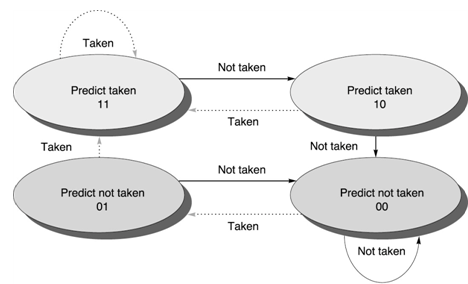
\includegraphics[width=1\textwidth]{figures/automato.png}
	\caption{Aut\^{o}mato finito descreve o comportamento do preditor de saltos \cite{493986}.}
	\label{fig:Fig_automato}
\end{figure}

\begin{figure}[ht]
	\centering
	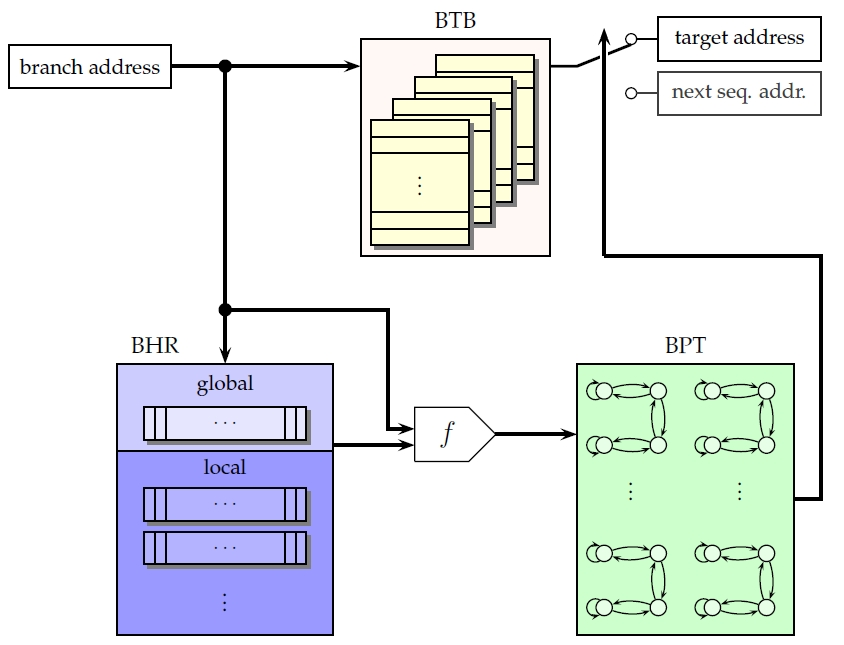
\includegraphics[width=.5\textwidth]{figures/btu.jpg}
	\caption{Unidade de predi\c{c}\~{a}o de saltos \cite{Jean-Pierre06predictingsecret}.}
	\label{fig:Fig_btu}
\end{figure}

\subsubsection*{Medi\c{c}\~{a}o direta de tempo}

A m\'{a}quina de estados que descreve as poss\'{i}veis decis\~{o}es da BTU possui um n\'{u}mero finito de estados; logo, o algoritmo que a descreve \'{e} determin\'{i}stico. O advers\'{a}rio pode assumir que a implementa\c{c}\~{a}o do RSA utilizou S\&M (\textit{Square-and-Multiply exponentiation algorithm}) e MM (\textit{Montgomery Multiplication algorithm} \cite{ECCBook_HankersonVanstone2004, 1197338}) e o BTU possui um aut\^{o}mato finito de apenas dois estados: salto tomado ou n\~{a}o tomado.

Seja $d$ a chave privada, vamos supor que o advers\'{a}rio conhece seus $i$ primeiros bits e est\'{a} tentando determinar $d_{i}$. Para qualquer mensagem $m$, o advers\'{a}rio pode simular as primeiras $i$ itera\c{c}\~{o}es e obter um resultado intermedi\'{a}rio que ser\'{a} a entrada da $(i+1)-$\textit{\'{e}sima} itera\c{c}\~{a}o. Ent\~{a}o ele gera quatro conjuntos distintos tais que:

\begin{align} \notag
	M_{1} = \left\lbrace m\ \vert\ d_{i} = 1 \rightarrow m\ causa\ missprediction\ durante\ MM\right\rbrace \\ \notag
	M_{2} = \left\lbrace m\ \vert\ d_{i} = 1 \rightarrow m\ causa\ hit\ durante\ MM\ \ \ \ \ \ \ \ \ \ \ \ \ \ \ \ \ \ \ \ \right\rbrace \\ \notag
	M_{3} = \left\lbrace m\ \vert\ d_{i} = 0 \rightarrow m\ causa\ missprediction\ durante\ MM\right\rbrace \\ \notag
	M_{4} = \left\lbrace m\ \vert\ d_{i} = 0 \rightarrow m\ causa\ hit\ durante\ MM\ \ \ \ \ \ \ \ \ \ \ \ \ \ \ \ \ \ \ \ \right\rbrace \\ \notag
\end{align}

O advers\'{a}rio calcula o tempo m\'{e}dio de execu\c{c}\~{a}o na multiplica\c{c}\~{a}o de Montgomery em cada conjunto $M_{i}$. Sendo $d_{i} = t, t \in \left\lbrace 0,1\right\rbrace $, a diferen\c{c}a dos tempos m\'{e}dios de execu\c{c}\~{a}o para o mesmo valor correto $t$ ser\~{a}o muito mais significativas do que a obtida dos outros dois conjuntos, pois, para o valor incorreto, os valores de tempo de cada multiplica\c{c}\~{a}o ter\~{a}o um caracter aleat\'{o}rio. Esse \'{e} o mesmo processo estat\'{i}stico da an\'{a}lise diferencial de pot\^{e}ncia. Portanto, se a diferen\c{c}a entre os tempos m\'{e}dios de $M_{1}$ e $M_{2}$ for muito mais significativa do que $M_{3}$ e $M_{4}$, ent\~{a}o o palpite correto \'{e} $d_{i} = 1$, e $d_{i} = 0$ caso contr\'{a}rio. 

Nesse ataque o advers\'{a}rio precisa saber de antem\~{a}o o estado do BPU antes do algoritmo de decripta\c{c}\~{a}o ser iniciado. Uma possibilidade de simples implementa\c{c}\~{a}o, por\'{e}m menos eficiente, seria realizar a an\'{a}lise supondo cada um dos quatro estados iniciais. A segunda abordagem consiste em for\c{c}ar o estado inicial do BPU de modo que nenhum endere\c{c}o de salto esteja no BTB. Essa abordagem ser\'{a} fundamentalmente a mesma utilizada em todos os ataques de predi\c{c}\~{a}o de salto listados a seguir.

\subsubsection*{For\c{c}ando BPU \`{a} mesma predi\c{c}\~{a}o assincronamente}

Unidades de processamento que permitem execu\c{c}\~{a}o concorrente de processos (SMT ou \textit{Simultaneous Multi-Threading} \cite{Silberschatz2004}) permitem que um advers\'{a}rio execute um processo espi\~{a}o simultaneamente ao programa de encripta\c{c}\~{a}o. Dessa forma, o advers\'{a}rio pode fazer com que o valor previsto dos saltos do encriptador nunca estejam no BTB; conseq\"{u}entemente, sempre ocorrer\'{a} um \textit{missprediction} quando o resultado correto, segundo a previs\~{a}o, seria que o salto fosse tomado. Comparado ao processo anterior, a an\'{a}lise diferencial seria similiar exceto pelo fato de que $d_{i} = 1$ em caso de \textit{hit} e $d_{i} = 0$ em caso de \textit{missprediction} durante o c\'{a}lculo de $m^{2} \bmod N$.

O processo espi\~{a}o remover do BTB o endere\c{c}o alvo de salto dos seguintes modos:
\begin{enumerate}
	\item (\textit{Total Eviction Method}: todas as entradas do BTB s\~{a}o expulsas.
	\item (\textit{Partial Eviction Method}): um conjunto de entradas do BTB \'{e} expulso.
	\item (\textit{Single Eviction Method}): apenas endere\c{c}o de interesse \'{e} expulso da tabela.
\end{enumerate}

Obviamente o primeiro m\'{e}todo \'{e} o de mais simples implementa\c{c}\~{a}o (assumindo que sejamos capazes de esvaziar todo o BTB entre duas itera\c{c}\~{o}es da exponencia\c{c}\~{a}o). O diferencial desse ataque \'{e} o advers\'{a}rio n\~{a}o ter que saber detalhes de implementa\c{c}\~{a}o da BPU para ser capaz de criar o processo espi\~{a}o e determinar quais s\~{a}o os bits da chave secreta.

\begin{figure}[ht]
	\centering
	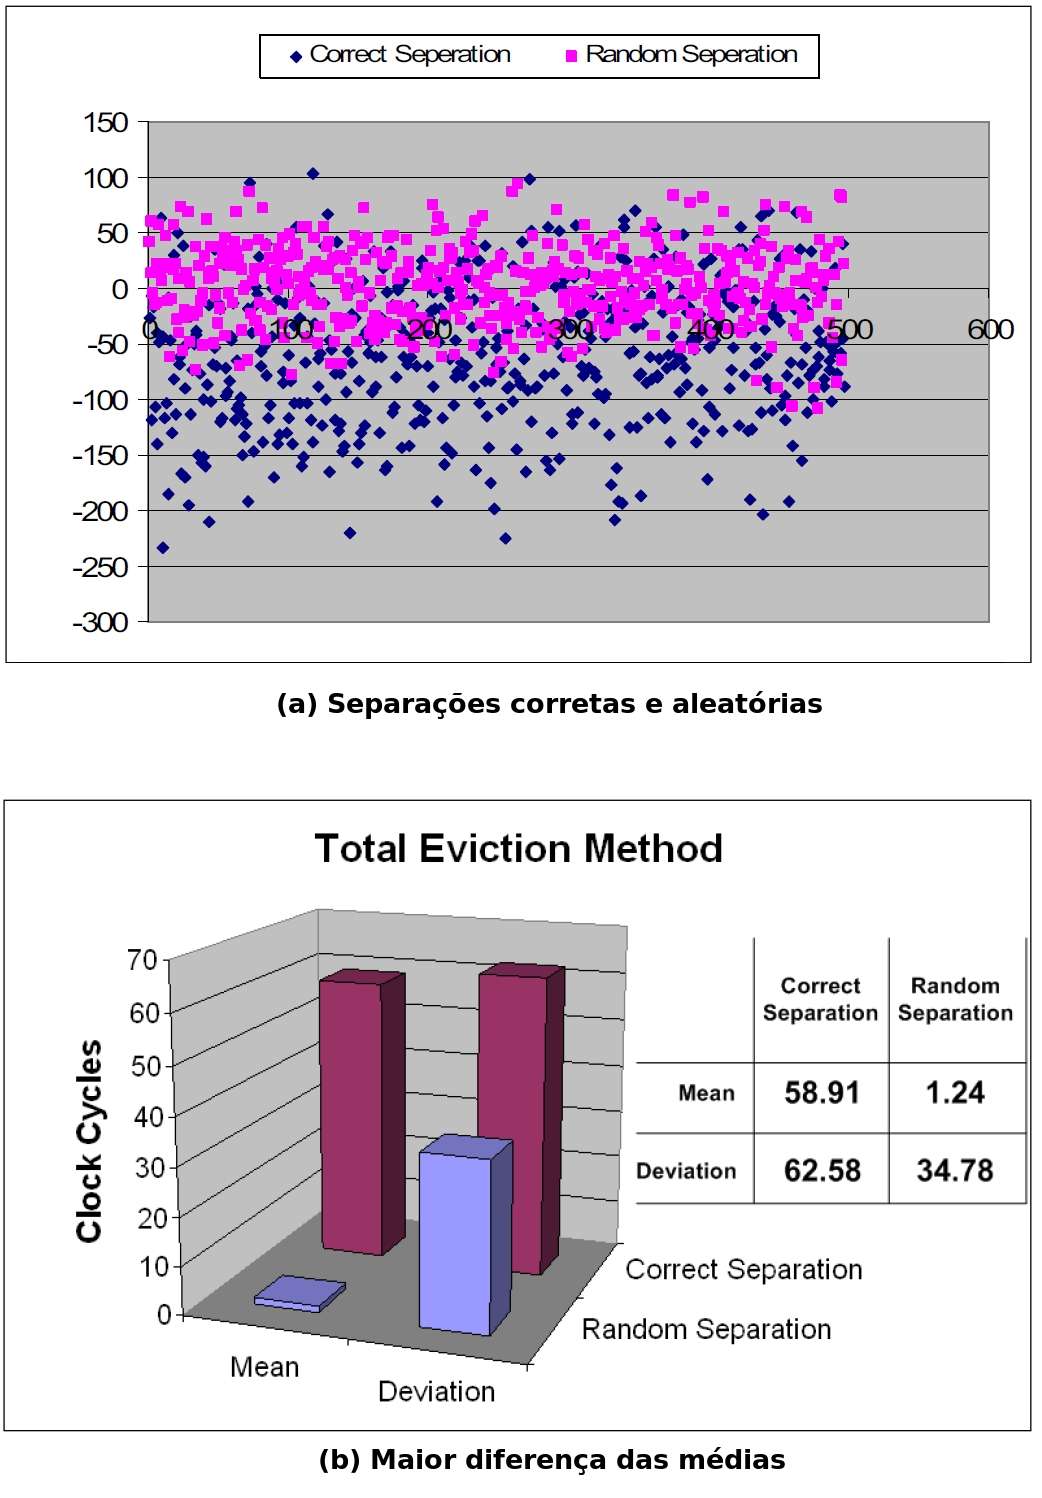
\includegraphics[width=.7\textwidth]{figures/totaleviction.jpg}
	\caption{Resultados pr\'{a}ticos do \textit{Total Eviction Method} \cite{Jean-Pierre06predictingsecret}.}
	\label{fig:Fig_totaleviction}
\end{figure}

Esse ataque foi aplicado sobre uma implementa\c{c}\~{a}o do RSA em OpenSSL vers\~{a}o 0.9.7, rodando sob uma workstation RedHat 3. Foram gerados 10 milh\~{o}es de blocos de mensagens aleat\'{o}rias e chaves aleat\'{o}rias de $512$ bits. As mensagens foram encriptadas e separadas segundo os crit\'{e}rios acima, sendo assumido como tomado o salto do pr\'{o}ximo bit desconhecido.
       
Na Figura ~\ref{fig:Fig_totaleviction} (a), o eixo $x$ corresponde aos bits do expoente de 2 at\'{e} 511, sendo que cada coordenada $x_{i}$ apresenta os valores das m\'{e}dias das separa\c{c}\~{o}es correta e a m\'{e}dia das separa\c{c}\~{o}es aleat\'{o}rias, denotadas respectivamente por $\mu_{Y_{i}}$ e $\mu_{X_{i}}$. Analizando todos os pares $(\mu_{Y_{i}}, \mu_{X_{i}})$, o advers\'{a}rio verifica  qual deles teve a diferen\c{c}a mais significativa (Figura ~\ref{fig:Fig_totaleviction} (b)) e utiliza seus respectivos desvios padr\~{o}es para determinar o desvio da diferen\c{c}a das m\'{e}dias

\begin{align}\notag
    \mu_{Z} &= \mu_{Y} - \mu_{X} = 58.91 - 1.24 = 57.67\\\notag
    \sigma_{Z} &= \sqrt{ \sigma_{Y}^{2} + \sigma_{X}^{2}} = \sqrt{ 62.58^{2} - (34.78)^{2}} = 71.60\\ \notag
\end{align}

Sempre que o advers'{a}rio encontrar $Z > 0$, ele ir\'{a} supor que seu palpite do valor do \textit{bit} foi correta. O grau de certeza que o advers\'{a}rio pode ter nessas decis\~{o}es pode ser medido atrav\'{e}s da probabilidade:

\begin{align}
    Pr[Z > 0] = \phi(\dfrac{0 - \mu_{Z}}{\sigma_{Z}}) = \phi(-0.805) = 0.79\notag
\end{align}

Portanto, a probabilidade de suas decis\~{o}es estarem corretas para essas medidas \'{e} de quase 80\%, viabilizando o advser\'{a}rio obter o restante da chave por for\c{c}a bruta.

\subsection{Canal lateral de potência}

\subsubsection{Características gerais}
Em um ataque sobre o canal lateral de pot\^{e}ncia, o advers\'{a}rio analisa sutis varia\c{c}\~{o}es no consumo de energia el\'{e}trica de um dispositivo cujo \textit{hardware} implementa um algoritmo criptogr\'{a}fico (sensores RFID, \textit{smartcards}, \textit{SIM cards}, etc).

Opera\c{c}\~{o}es com dados sens\'{i}veis geram alter\c{c}\~{o}es na corrente ou tens\~{a}o da alimenta\c{c}\~{a}o do dispositivo, permitindo extrair parcialmente (ou mesmo integralmente) a chave criptogr\'{a}fica e outras informa\c{c}\~{o}es  sens\'{i}veis. O primeiro ataque dessa natureza foi apresentado por \cite{Kocher:1999:DPA:646764.703989}, tamb\'{e}m autor da c\'{e}lebre pesquisa precursora sobre \textit{time attacks} \cite{Kocher96}. 

\subsubsection{Ataque de potência simples (SPA)}
A tecnologia de semicondutores dominante em microprocessadores, mem\'{o}rias e dispositivos embarcados \'{e} a CMOS   \cite{sedra:1997}, sendo inversores l\'{o}gicos sua unidade b\'{a}sica de constru\c{c}\~{a}o. Como dispositivos utilizam fontes constantes de tens\~{a}o, a pot\^{e}ncia consumida varia de acordo com o fluxo de sinais nos componentes, e esses de acordo com as opera\c{c}\~{o}es realizadas. Se esse consumo de pot\^{e}ncia for monitorado com aux\'{i}lio de um oscilosc\'{o}pio poderemos estabelecer um rastro de consumo de pot\^{e}ncia (\textit{power trace}) a cada ciclo do dispositivo.

\subsubsection{An\'{a}lise simples de pot\^{e}ncia sobre ECDSA}
Uma das rotinas mais executadas em dispositivos que utilizam ECC s\~{a}o os algoritmos de assinatura digital de curvas el\'{i}pticas (\textit{ECDSA} ou \textit{Elliptic Curve Digital Signature Algorithm}), tendo como opera\c{c}\~{a}o central a multiplica\c{c}\~{a}o de um ponto por um escalar (Algoritmo 9).

\floatname{algorithm}{Algoritmo}
\begin{algorithm}[H]
\caption{Binary NAF method for scalar multiplication}
\begin{algorithmic}
    \REQUIRE $P \in E(\mathbb{F}_p), k \in \mathbb{N}$
    \ENSURE $Q = kP \in E(\mathbb{F}_p)$
    \STATE $(k_{l-1}, k_{l-2}, ..., k_{1}, k_{0}) \leftarrow NAF(k)$
    \STATE $Q \leftarrow \infty$
    \FOR {$j \leftarrow l - 2$ \TO $0$}
        \STATE $Q \leftarrow 2Q$
        \IF {$k_{i} = 1$}
            \STATE $Q \leftarrow Q + P$
        \ENDIF
        \IF {$k_{i} = -1$}
            \STATE $Q \leftarrow Q - P$
        \ENDIF
    \ENDFOR
    \RETURN $Q$
    \end{algorithmic}
\end{algorithm}

\begin{figure}[ht]
	\centering
	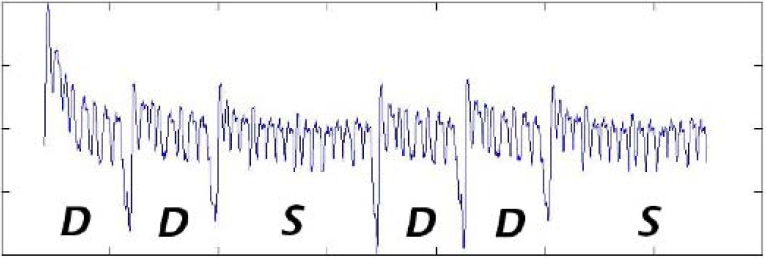
\includegraphics[width=.8\textwidth]{figures/spa1.jpg}
	\caption{Consumo de pot\^{e}ncia durante c\'{a}lculo de $kP$ \cite{ECCBook_HankersonVanstone2004}.}
	\label{fig:Fig5}
\end{figure}

O que torna a forma n\~{a}o adjacente de $k$ mais interessante do que sua representa\c{c}\~{a}o bin\'{a}ria \'{e} o fato da $NAF(k)$ possuir apenas $1/3$ de d\'{i}gitos n\~{a}o nulos. Conseq\"{u}entemente uma quantidade muito menor de adi\c{c}\~{o}es (linhas $04$ e $05$ do Algoritmo 8) s\~{a}o efetuadas.

Entretanto um advers\'{a}rio que soubesse que o dispositivo implementa um algoritmo \textit{ECDSA} poderia monitorar o consumo de pot\^{e}ncia do dispositivo utilizando um oscilosc\'{o}pio, obtendo o gr\'{a}fico mostrado na Figura~\ref{fig:Fig5}. No Algoritmo 9, vemos que adi\c{c}\~{o}es s\~{a}o realizadas apenas quando $k_{i} \neq 0$; logo, uma maior quantidade de pot\^{e}ncia \'{e} despendida para d\'{i}gitos n\~{a}o nulos. Portanto os intervalos curtos denominados $D$ correspondem a itera\c{c}\~{o}es em que $k_{i} = 0$, enquanto intervalos longos denominados $S$ correspondem a itera\c{c}\~{o}es em que $k_{i} \neq 0$. Essa informa\c{c}\~{a}o torna vi\'{a}vel descobrir a chave atrav\'{e}s de ataques por for\c{c}a bruta, pois apenas $1/3$ dos d\'{i}gitos s\~{a}o n\~{a}o nulos.

A solu\c{c}\~{a}o mais simples contra SPA consiste em inserir opera\c{c}\~{o}es redundantes no algoritmo de multiplica\c{c}\~{a}o (Algoritmo 10), de modo que a seq\"{u}\^{e}ncia de opera\c{c}\~{o}es elementares envolvidas sejam realizadas em igual propor\c{c}\~{a}o. Comparando o novo \textit{power trace} obtido (Figura~\ref{fig:Fig7}) n\~{a}o \'{e} poss\'{i}vel diferenciar adi\c{c}\~{o}es de multiplica\c{c}\~{o}es.

\floatname{algorithm}{Algoritmo}
\begin{algorithm}[H]
\caption{Binary NAF method for scalar multiplication resistant to SPA}
\begin{algorithmic}
    \REQUIRE $P \in E(\mathbb{F}_p), k \in \mathbb{N}$
    \ENSURE $Q = kP \in E(\mathbb{F}_p)$
    \STATE $(k_{l-1}, k_{l-2}, ..., k_{1}, k_{0}) \leftarrow NAF(k)$
    \STATE $Q \leftarrow \infty$\\
    \FOR {$i = l-1$ \TO $0$}
        \STATE $Q_{0} = 2Q_{0}$
        \STATE $Q_{1} = Q_{0} + P$
        \STATE $Q_{0} = Q_{k_{i}}$
    \ENDFOR
    \RETURN $Q$
    \end{algorithmic}
\end{algorithm}

\begin{figure}[ht]
	\centering
	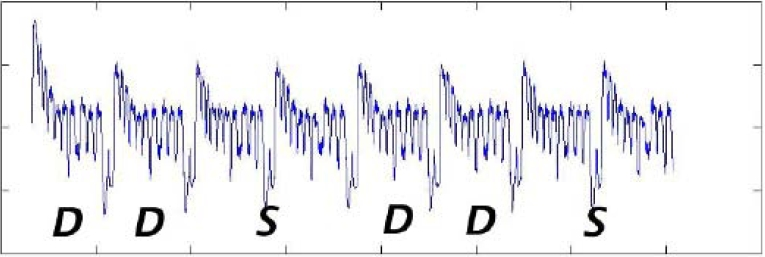
\includegraphics[width=.8\textwidth]{figures/spa2.jpg}
	\caption{Consumo de pot\^{e}ncia durante c\'{a}lculo de $kP$ \cite{ECCBook_HankersonVanstone2004}.}
	\label{fig:Fig7}
\end{figure}

\subsubsection{Ataque de potência diferencial (DPA)}
Quando a varia\c{c}\~{a}o do consumo de pot\^{e}ncia n\~{a}o \'{e} sens\'{i}vel o suficiente em rela\c{c}\~{a}o as opera\c{c}\~{o}es executadas por um dispositivo, o advers\'{a}rio pode monitorar como o consumo varia em rela\c{c}\~{a}o ao valor de uma determinada vari\'{a}vel. Nesse ataque, primeiramente detectamos uma vari\'{a}vel $V$, influenciada, durante um processo de decripta\c{c}\~{a}o ou assinatura digital, por um texto $m$ e uma por\c{c}\~{a}o desconhecida  da chave privada. A partir disso, definimos a fun\c{c}\~{a}o de sele\c{c}\~{a}o $V = f(k',m)$.

O advers\'{a}rio ent\~{a}o coleta milhares de \textit{power traces}, determinando indutivamente todos os bits que comp\~{o}em a chave privada atrav\'{e}s do c\'{a}lculo da derivada dessa fun\c{c}\~{a}o. Para cada bit $k'_{i}$ corretamente previsto obtemos uma derivada n\~{a}o nula para os valores de $k'$ e $m$, caso contr\'{a}rio a derivada \'{e} nula. O processo \'{e} repetido at\'{e} que cada $k'_{i}$ seja determinando \cite{ECCBook_HankersonVanstone2004}. Esse modelo de ataque \'{e} conhecido como An\'{a}lise Diferencial de Pot\^{e}ncia (DPA ou \textit{Differential Power Analysis}).


\subsection{An\'{a}lise diferencial de pot\^{e}ncia sobre ECDSA}
Ainda que o Algoritmo 10 tenha sido adotado, podemos aplicar um DPA sobre o processo de ECDSA. 

Determinada uma vari\'{a}vel $V$ cujo valor influencie o consumo de pot\^{e}ncia e uma fun\c{c}\~{a}o de sele\c{c}\~{a}o $f$ tal que $V = f(k', m)$ o advers\'{a}rio coleta milhares de \textit{power traces}, estima o tamanho que a por\c{c}\~{a}o $k'$ ocupa na chave privada e separa os dados coletados em dois grupos de acordo com o valor previsto de $V$.

No algoritmo de multiplica\'{c}\~{a}o de pontos da curva el\'{i}ptica (Algoritmo 1.6), suponha que Eve colete \textit{power traces} durante os c\'{a}lculos $kP_{1} , kP_{2} , ..., kP_{r}$ . Como $P_{1} , P_{2} , ..., P_{r}$ s\~{a}o p\'{u}blicos, ele precisa determinar apenas $k$.

\begin{center}
    \begin{tabular}{|c|c|c|c|c|}
	    \hline
		    \   & $Q_{0}$  & $Q_{0}$ & $k_{t-1}$ & $Q_{0} \leftarrow Q_{k_{t-1}}$\\
	    \hline
	        $1$ & $\infty$ &     $P$ &       $1$ & $P$\\
	    \hline
		    $2$ & ... & ... & ... & ...\\
	    \hline
		    $3$ & ... & ... & ...& ... \\
	    \hline
		    ... & ... & ... & ...& ... \\
	    \hline
    \end{tabular}

    Tabela 1.2. $k = (1, k_{t-2}, k_{t-3}, ..., k_{1}, k_{0})$.
\end{center}

Dado $Q_{0} = \infty$, o passo 2.1 \'{e} trivial e pode ser disting\"{u}ir da de uma opera\c{c}\~{a}o n\~{a}o trivial
atrav\'{e}s do power trace, logo o advers\'{a}rio pode facilmente identificar o bit mais a esquerda cujo valor e 1. Tomando $k_{t-1}= 1$, na segunda itera\c{c}\~{a}o do algoritmo temos que $Q_{0} = 2P$ (se $k_{t-2} = 0$) ou $Q_{0} = 3P$ (se $k_{t-2} = 1$).

\begin{center}
    \begin{tabular}{|c|c|c|c|c|}
	    \hline
		    \   & $Q_{0}$  & $Q_{0}$ & $k_{t-1}$ & $Q_{0} \leftarrow Q_{k_{t-1}}$\\
	    \hline
	        $1$ & $\infty$ &     $P$ &       $1$ & $P$\\
	    \hline
		    $2$ & $2P$ & $4P$ & $\color{blue}{?}$ & $\color{blue}{?}$ \\
	    \hline
		    $3$ & ... & ... & ...& ... \\
	    \hline
		    ... & ... & ... & ...& ... \\
	    \hline
    \end{tabular}

    Tabela 1.3. $k = (1, k_{t-2}, k_{t-3}, ..., k_{1}, k_{0})$.
\end{center}

Conseq\"{u}entemente, na terceira itera\c{c}\~{a}o, o valor $4P$ ser computado apenas se $k_{t-2} = 0$. Definindo $k' = k_{t-2}$ e $m = P_{i}$ ($i$-\'{e}simo bit do ponto $4P = (4P_{1} , 4P_{2} , ..., 4P_{i} , ..., 4P_{r} , )$), a fun\c{c}\~{a}o seletora calcula o valor do bit $4P_{i}$.

\begin{center}
    \begin{tabular}{|c|c|c|c|c|}
	    \hline
		    \   & $Q_{0}$  & $Q_{0}$ & $k_{t-1}$ & $Q_{0} \leftarrow Q_{k_{t-1}}$\\
	    \hline
	        $1$ & $\infty$ &     $P$ &       $1$ & $P$\\
	    \hline
		    $2$ & $2P$ & $4P$ & $\color{red}{0}$ & $2P$ \\
	    \hline
		    $3$ & $\color{red}{4P}$ & $6P$ & ...& ... \\
	    \hline
		    ... & ... & ... & ...& ... \\
	    \hline
    \end{tabular}

    Tabela 1.4. $k = (1, \color{red}{0}$$,\ $$k_{t-3}, ..., k_{1}, k_{0})$.
\end{center}

Se o gr\'{a}fico do consumo de pot\^{e}ncia da fun\c{c}\~{a}o apresentar picos, ent\~{a}o $k_{t-2} = 0$, caso contr\'{a}rio $k_{t-2} = 1$.
Esse processo \'{e} repetido at\'{e} todos os bits de $k$ serem determinados \cite{ECCBook_HankersonVanstone2004}.

Se a curva el\'{i}ptica for gerada sobre um $\mathbb{F}_{p}$ de caracter\'{i}stica superior a 3, podemos usar um sistema misto de representa\c{c}\~{a}o de coordenadas no qual $P$ seja representado em um sistema de coordenadas afins, enquanto $Q_{0}$ e $Q_{1}$ s\~{a}o representados em coordenadas jacobianas \cite{ECCBook_HankersonVanstone2004}.

Se $P = (x,y)$ no sistema afim, ap\'{o}s a primeira atribui\c{c}\~{a}o $Q_{1} \leftarrow P$ ter\'{i}amos $ Q_{1} = (x : y : 1)$. Ent\~{a}o, $Q_{1}$ seria aleatorizado com $(\lambda^{2}x, \lambda^{3}y, \lambda)$ e o algoritmo procederia como o usual. Desse modo o advers\'{a}rio estaria impedido de realizar predi\c{c}\~{o}es baseadas no valor de um bit espec\'{i}fico $4P_{i}$ em sistemas de coordenadas jacobianas aleatorizadas.

\subsubsection{High-order DPA}
Uma variação do ataque de potência diferencial é o \textit{high-order} DPA (HODPA), esse ataque é baseado em um conjunto de propriedades estatísticas do sinal de potência. Para obter uma melhor taxa de acerto dos \textit{bits} da chave é necessário uma quantidade maior de amostras. Além disso, existe uma complexidade maior durante a implementação desse ataque \cite{benedikt:2009:228}.

Um ponto importante a ser observado é que esse ataque possui a capacidade de sobrepor a resistência de uma contramedida de \textit{masking} e obter os \textit{bits} da chave. Isso é possível pela análise tanto do valor mascarado como da própria máscara criando uma relação entre ambos. Um problema encontrado na utilização desse ataque é a identificação de em qual tempo é necessário obter o sinal referente ao valor mascarado ou a máscara.

\subsubsection{Template attacks}
O ataque que será apresentado, \textit{Template Attack} (TA), utiliza amostras de potência elétrica para executar uma análise na tentativa de obter os \textit{bits} da chave privada. O mesmo é considerado o mais poderoso dentre os ataques de potência diferencial. Existe uma divisão em duas fases do ataque sendo: a fase de construção e a fase de correlação. A primeira gera um \textit{template} de um padrão obtido no dispositivo alvo. Na segunda é analisada a correlação entre o \textit{template} gerado e as amostras obtidas durante a execução do dispositivo \cite{ozgen:2016}. Esse ataque pode ser combinado com algoritmos de classificação para diferenciar valores da chave e o restante como é proposto no trabalho de \cite{ozgen:2016}. Uma outra opção é a utilização de algoritmos de reconhecimento de padrões com aprendizado de máquina.


\section{Ataques e contramedidas para encriptação simétrica e hash}
\subsection{Utilização de CPA em implementação do AES}

\subsection{Ataques por canal lateral de tempo}

Ataques de latência de \emph{cache} e verificação de MAC:
ataques no AES e comparação de strings.

Ataques a HMAC baseado em funções de hash construídas por cifras de bloco.

Cube attacks em cifras de bloco.

\subsection{Contramedida de mascaramento}



\subsection{Oráculo de preenchimento}

Ataque de Vaudenay no modo CBC.

\section{Ataques e contramedidas para ECC}
\subsection{Níveis em que os ataques SCA podem ser aplicados}

% 1 parag. p/ explicar a figura e discutir brevemente exemplos de ataques em cada nível.

\begin{figure}[h!tb]
	\centering   %height=0.20\textheight
	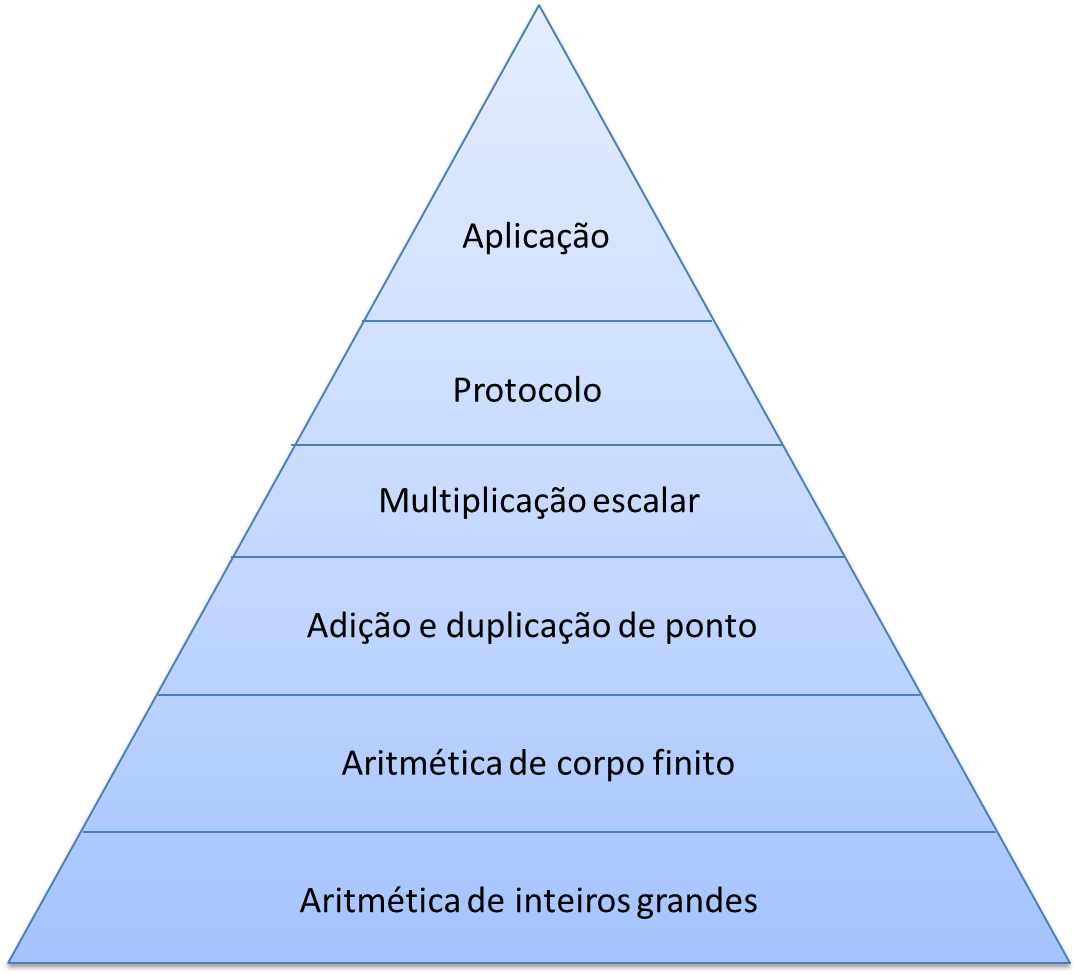
\includegraphics[width=0.9\textwidth]{figures/piramide_ECC.png}
	\caption{
		Pirâmide de implementação de criptografia baseada em curvas elípticas (ECC). Qualquer uma destas camadas pode ser vulnerável a ataques pode canais laterais.
	}
	%\vspace{.5mm}
	\label{fig:pyramid-ecc}
\end{figure}

A implementação de protocolos criptográficos baseados em curvas elípticas depende da existência de implementações de um conjunto de operações básicas, tais como: multiplicação de ponto por escalar, adição e duplicação de ponto, aritmética de corpo finito e aritmética de inteiros grandes. Protocolo criptográficos podem ser implementados a partir destas operações primitivas, os quais por sua vez possibilitam implementar um aplicação. A~\Cref{fig:pyramid-ecc} ilustra tais operações como níveis/camadas de uma pirâmide, onde a implementação de uma operação em uma camada depende apenas da existência de funcionalidades na camada imediatamente inferior\footnote{Operações adicionais podem ser necessárias para alguns protocolos, como a aritmética modular cujo módulo é o número de pontos da curva. Além disso, curvas elípticas definidas sobre corpos finitos binários dependem da aritmética em polinômios grandes.}.

A representação em pirâmide entretanto esconde a interdependência que existe entre as operações. Na prática, bibliotecas de primitivas e protocolos criptográficos há interação em todos os níveis da pirâmide, pois tais interações ou interdependências são relevantes para desempenho, e em alguns casos, segurança. 

Em uma implementação de uma dada aplicação, qualquer um dos níveis da pirâmide da figura acima pode estar vulnerável a ataques por canais laterais. Com relação ao canal de tempo, por exemplo, se uma operação não é de tempo constante com a relação à chave ou valores intermediários dependentes da chave, então todas as operações em níveis superiores à esta, bem como protocolo e aplicação vazam por diferenças potencialmente observáveis de tempo tais informações, as quais podem, a princípio, serem exploradas pelo atacante e portanto vulneráveis.

% (dentre aquelas entre a aritmética de inteiros grandes até a multiplicação escalar)

%\subsection{Transferência de chaves}
%\erick[inline]{TODO: Transferência da chave entre diferentes memórias}
%\erick[inline]{TODO: processamento da chave fora do algoritmo criptográfico. Ref. sobre um SCA bem sucedido deste tipo: Witteman, M. (2013). Secure Application Programming in the Presence of Side Channel Attacks.\cite{Witteman2013_PatternsAppsecSCA}. Autor demonstra um ataque à verificação de paridade da chave na biblioteca GnuPG.}

\subsection{Ataques de tempo e SPA ao algoritmo double-and-add-not-always}

\subsubsection{Ataque de tempo ao algoritmo double-and-add-not-always}
Considerando que o SPA de tempo se baseia na variação de tempo do algoritmo dependendo do valor da chave é possível realizar o ataque de tempo em algoritmos que não executam em tempo constante. Nesse caso, a maneira mas simples de observar uma implementação insegura é a presença de branchs condicionais. Um exemplo é no caso de um algoritmo possuir uma instrução de \textit{if} onde ele apenas executa as operações contidas nessa instrução dependendo dos \textit{bits} da chave privada.

Nesse contexto podemos observar um ataque de tempo aplicado a uma implementação do RSA por \cite{Kocher96}, esse foi o primeiro ataque de tempo proposto. O mesmo pode ser aplicado a implementações de curvas elípticas considerando que basicamente o atacante faz a análise do tempo de execução do algoritmo, tenta advinhar os \textit{bits} da chave e valida se o resultado está correto.

No trabalho de \cite{danger2013synthesis} é descrito um ataque à um implementação genérica de ECSM. O mesmo segue os seguintes passos: primeiramente o atacante coleta o tempo de execução de diferentes ECSMs com o mesmo escalar e diferentes pontos base. Para cada ECSM, ele simula a computação usando um simulador de software com exatamente a mesma implementação do chip alvo, "chutando" o valor do bit $i$ do escalar. 

Agora suponha, sem perda de generalidade, que a hipótese é de que o valor do \textit{bit} é $0$.  Ele separa os diferentes tempos de execução em dois conjuntos, $S_1$ e $S_2$. Caso uma redução é necessária ao final da execução o tempo obtido é armazenado em $S_2$, senão é armazenado em $S_1$. Após toda a execução é feita uma média dos tempos armazenados em $S_1$ e $S_2$, e se a diferença entre as médias for aproximadamente o tempo de execução da redução portanto a hipótese estava correta.

\begin{comment}
\erick[inline]{Lucas: ver o comentario no fonte. Converter comentario em texto}.

1.	Ataque SPA à alg. ECSM binário left-to-right (Dbl-and-Add not Always)
	a.	Se impl não é de tempo constante, então é possível realizar ataque de tempo.
		i.	P.ex., se usa if and else, então pode-se determinar a cada iteração qual bloco, if ou else, é tomado.
	b. O ataque de tempo em~\cite{Kocher96} ao RSA pode ser aplicado no contexto de ECC. Segue abaixo a ideia do ataque (baseada no survey de ~\cite{Danger2013}, Sec. 3.2.1).
	
	O atacante coleta o tempo de execução de diferentes ECSMs com o mesmo escalar e diferentes pontos base. Para cada ECSM, ele simula a computação usando um simulador de software com exatamente a mesma implementação do chip alvo, "chutando" o valor do bit $i$ do escalar. Suponha, sem perda de generalidade, que a hipótese é de que o valor do bit é 0.  Ele separa os diferentes tempos de execução em dois conjuntos, S_1 e S_2. Se, a iteração
	
	%TODO: CONT HERE
	

[Kocher96] Kocher, P.C.: Timing attacks on implementations of Diffie–
Hellman, RSA, DSS, and other systems. In: Proceedings of CRYPTO’96, LNCS, vol. 1109. Springer, Berlin, pp. 104–113
(1996)
\end{comment}

\subsubsection{Ataque SPA ao algoritmo double-and-add-not-always}
O algoritmo \textit{double-and-add-not-always} executa em tempo constante, contudo o ataque SPA (com ou sem power model) pode ser aplicado para distinguir os padrões no \textit{trace} das iterações com apenas DBL (onde o \textit{bit} da chave é igual à $0$) daquelas com DBL+ADD (com \textit{bit} da chave igual à $1$). Um ataque deste tipo segmenta/divide o \textit{trace} de potência de uma execução do ECSM em \textit{subtraces}, cada uma contendo uma operação de ponto (ADD ou DBL). 

Se o tempo de execução de uma operação de ADD for diferente do tempo de DBL, então o comprimento dos \textit{subtraces} revela onde estão os ADDs e consequentemente os bits do escalar. Se o tempo da operação ADD e o tempo da DBL forem iguais, e uma fórmula unificada para ADD and DBL é utilizada, então, se for aplicada correlação (coeficiente de correlação de Pearson) entre todos os pares de \textit{subtraces}, o resultado será que a correlação será mais alta para os pares de subtraces cuja operação correspondente é a mesma (i.e., (ADD,ADD) ou (DBL,DBL)), identificando portanto as operações de ponto e consequentemente os \textit{bits} do escalar.

Mesmo sendo que a implementação seja vulnerável a SPA é desejável que execute em tempo constante, o que cria uma base para a implementação de outras contramedidas. Portanto, é necessário observar que para executar o ataque SPA são requisitados equipamentos para medir a potência como um osciloscópio, além disso, o ataque por tempo possui simplicidade em comparação com SPA sendo que apenas é necessária a capacidade de verificar o tempo de execução do algoritmo e inserir entradas distintas.

\begin{comment}
\erick[inline]{Lucas: ver o comentario no fonte. Converter comentario em texto}.

b.	Se é de tempo constante, SPA (com ou sem power model) pode ser aplicado para distinguir os padrões no trace das iterações com apenas DBL (bit=0) daquelas com DBL+ADD (bit=1). Um ataque deste tipo segmenta/divide o trace de potencia de uma execucao do ECSM em subtraces, cada um contendo uma operacao de ponto (ADD ou DBL). Se as tempo(ADD) != tempo(DBL), então o comprimento dos subtraces revela onde estão os ADDs e consequentemente os bits do escalar. Se tempo(ADD) == tempo(DBL) e uma formula unificada para ADD and DBL é utilizada, então, se for aplicada correlação (coeficiente de correlacao de Pearson) entre todos os pares de subtraces, o resultado será que a correlação será mais alta para os pares de subtraces cuja operação correspondente é a mesma (i.e., (ADD,ADD) ou (DBL,DBL)), identificando portanto as operações de ponto e consequentemente os bits do escalar.
\end{comment}

%TODO 2. Argumentar que é fortemente desejável que as implementações sejam de tempo constante, de modo a ser uma base para a implementação das outra contramedidas para power analysis.

\subsection{Double-and-add-always algorithm of Coron~\cite{Coron1999}}

\begin{comment}
\erick[inline]{Lucas: traduzir esta secao}
\end{comment}

O algoritmo {\it double-and-add-always} de \cite{Coron1999} (Algoritmo 11) utiliza uma adição de ponto falsa conhecida como \textit{dummy point addition} quando o \textit{bit} escalar $k_i$ é $0$, tornando a sequência de operações computadas durante a multiplicação escalar independente do valor do escalar.

\begin{algorithm}[h] %\scriptsize %\footnotesize
	\caption{\small{\textit{Double-and-add always} algorithm resistant against SPA}}
	\label{Double-and-add-Coron}
	\begin{algorithmic}[1]
		\REQUIRE  Point $\textbf{P} \in E(\mathbb{F}_q),$ $k=(k_{n-1},\ldots,k_1,k_0)_2 \in \mathbb{N}$
		\ENSURE  $Q=[k] \cdot P$\\
		\STATE $R_0\leftarrow P_{\infty}$   \\
		\FOR{$i$ \textbf{from} $n-1$ \textbf{to} $0$} 
		\STATE $R_0\leftarrow 2R_0$  \\
		\STATE $R_1\leftarrow R_0+P$\\ \label{Paso_R_1_Double-and-add-Coron}
		\STATE $R_0\leftarrow R_{k_i}$\label{Step5Double-and-add-Coron} \\
		\ENDFOR
		\STATE return $R_0$\\
	\end{algorithmic}
\end{algorithm}

Portanto o adversário não consegue, em princípio, advinhar o valor do \textit{bit} $k_i$ por SPA. Uma desvantagem desse método é a sua baixa eficiência. Ele requer $nA + nD$ operações no corpo, um aumento de $33\%$ nas operações do corpo em comparação a versão desprotegida binária do algoritmo \textit{left-to-right}.

\subsubsection{Fouque and Valette's Doubling Attack \cite{CHES:FouVal03}}\label{Fouque-Valette-DoublingAttack}
O ataque de duplicação de Fouque-Valette~\cite{CHES:FouVal03} é baseado no fato de que é possível detectar se dois valores intermediários são iguais quando o algoritmo calcula a multiplicação escalar para pontos escolhidos $P$ e $2P$. Diversos algoritmos protegidos contra SPA são vulneráveis ao ataque d eFouque e Valette's, como o algoritmo clássico \textit{left-to-right} binário, incluindo as variações do mesmo, como o \textit{double-and-add-always} de Coron.

No algoritmo de Coron \textit{double-and-add-always}, algoritmo (Algoritmo~\ref{Double-and-add-Coron}), a soma parcial é calculada da seguinte maneira: $S_m(P) = \sum_{i=1}^{m}k_{n-i}2^{m-i} P=\sum_{i=1}^{m-1}k_{n-i}2^{m-1-i}(2P)+k_{n-m}P= S_{m-1}(2P)+k_{n-m}P$. Então o resultado intermediário do algoritmo no passo $m$ quando a entrada for $P$ será igual ao resultado intermediário no passo $m-1$ quando a entrada for $2P$, se e somente se, $k_{n-m} = 0$. Portanto, um atacante pode obter o escalar secreto comparando a computação de duplicação no passo $m+1$ para $P$ e no passo $m$ para $2P$ para recuperar o bit $k_{n-m}$. Se ambas as computações forem idênticas, $k_{n-m} = 0$, senão $k_{n-m} = 1$. Isso mostrou que com apenas duas requisições de multiplicação escalar escolhidas pelo atacante, é possível recuperar todos os \textit{bits} do escalar.~\footnote{O atacante coleta um traço de energia para a computação de $kP$ e um para a computação de $k(2P)$. Para cada iteração $m=1,...,n$ ele executa o ataque como descrito e encontra $k_{n-m}$.}

\begin{comment}
The doubling attack of Fouque-Valette~\cite{CHES:FouVal03} is based on the fact that it is possible to detect if two intermediate values are equal when the algorithm computes the scalar multiplication for points chosen points $P$ and $2P.$ Several algorithms protected against SPA are vulnerable to Fouque and Valette's attack, such as the classic binary left-to-right algorithm, including those derived from it, such as Coron's double-and-add-always algorithm.

%In ~\textit{double-and-add-always} algorithm (Algorithm~\ref{Double-and-add-Coron}), the partial sums are computed as follows: $S_k(P) = \sum_{i=0}^{k}d_{n-i}2^{k-i} P=\sum_{i=0}^{k-1}d_{n-i}2^{k-1-i}(2P)+d_{n-k}P= S_{k-1}(2P)+d_{n-k}P$. So, the intermediate result of the algorithm at step $k$ when given input $P$ will be equal to the intermediate result at step $k-1$ when given input $2P$, if and only if, $d_{n-k}=0$. Therefore, an attacker can obtain the secret scalar by comparing the doubling computation at step $k+1$ for $P$ and at step $k$ for $2P$ to recover the bit $d_{n-k}.$ If both computations are identical, $d_{n-k}=0$, otherwise $d_{n-k}=1$.
In Coron's double-and-add-always algorithm (Algorithm~\ref{Double-and-add-Coron}), the partial sums are computed as follows: $S_m(P) = \sum_{i=1}^{m}k_{n-i}2^{m-i} P=\sum_{i=1}^{m-1}k_{n-i}2^{m-1-i}(2P)+k_{n-m}P= S_{m-1}(2P)+k_{n-m}P$. So, the intermediate result of the algorithm at step $m$ when given input $P$ will be equal to the intermediate result at step $m-1$ when given input $2P$, if and only if, $k_{n-m}=0$. Therefore, an attacker can obtain the secret scalar by comparing the doubling computation at step $m+1$ for $P$ and at step $m$ for $2P$ to recover the bit $k_{n-m}.$ If both computations are identical, $k_{n-m}=0$, otherwise $k_{n-m}=1$. It has been shown that with only two scalar multiplication requests chosen by the attacker, it is possible to recover all the bits of the scalar.~\footnote{The attacker collects one power trace for the computation of $kP$ and one for the computation of $k(2P)$. For each iteration $m=1,...,n$, he runs the attack as described and finds $k_{n-m}$.}
%%\vspace{-0.5cm}
\end{comment}


\subsection{Contramedidas}

% TODO: apresentar uma contramedida de cada vez entre subseções com ataques, mostrando como ela protege contra um determinado ataque.

\begin{comment} % === CONTRAMEDIDAS ===
	a.	CM1 - Scalar Randomization (SR)
	b.	CM2 - Proj. Coord. Randomization and Re-randomization (CRR)
	c.	CM3 - Point Blinding (PB) 
	d.	CM4 – Scalar Splitting (SS)
\end{comment}

\subsubsection{Scalar Randomization (SR)}
Essa contramedida é aplicada no início da multiplicação escalar, e é executada da seguinte maneira:
\begin{itemize}
    \item Aleatoriamente selecione $r\in_R \{0,1\}^n$, para um pequeno $n$. $n=32$ é um parâmetro razoável no quesito do \textit{trade-off} entre segurnaça/eficiência;
    \item Calcule $k' \rcv k + r |E|$;
    \item Utilize $k'$ no lugar de $k$.
\end{itemize}

O custo da aplicação dessa contramedida está ligado à geração dos \textit{bits} pseudo-aleatório, $n$ iterações da ECMS, as adições e multiplicações para calcular $k'$ e $n$ \textit{bits} da SRAM. Já no quesito eficiência é necessário verificar que é vulnerável a ataques de template online (OTA) \cite{BatinaChmielewski2014}, entre outros. 

\begin{comment}
	%	\begin{itemize}
	%\item 
	At the beginning of the scalar multiplication:
	\begin{enumerate}
		\item Randomly select $r\in_R \{0,1\}^n$, for a small $n$. $n=32$ seems to be a reasonable security/efficiency trade-off.
		\item Compute $k' \rcv k + r |E|$.
		\item Use $k'$ in place of $k$.
	\end{enumerate}
	
	%\item 
	\underline{Cost}: generate $n$ (pseudo-)random bits, $n$ iterations to the ECSM, MULs and ADDs to compute $k'$, $n$ bits of SRAM.\\
	%\item 
	
	\underline{Effectiveness}: vulnerable to Online Template Attacks (OTA) {[Batina,2014]}, among others.
	%	\end{itemize}

\end{comment}

\subsubsection{Projective Coordinates (Re-)Randomization (CR)~\cite{Coron1999}}
As coordenadas projetivas usadas em Montgomery Ladder são $(X : Z)$. Os passos para aplicar essa contramedida são:
\begin{itemize}
    \item Gerar um valor pseudo-aleatório $\lambda \mathbb{F}_p \backslash \{0\}$;
    \item Calcule $Z_2 \rcv \lambda$ and $X_2 \rcv u \cdot \lambda$, onde $u$ é a coordenada $x$ do ponto $P$ da entrada;
    \item Utilize $P'=(X_2:Z_2)$ no lugar de $P$.
\end{itemize}

Existe um custo de geração de $\ceil{log_2(p)}$ \textit{bits} aleatórios. Além disso, algumas vantagens ligadas a essa randomização das coordenadas como por exemplo a resistência à ataques online de template \cite{BatinaChmielewski2014}, pode ser aplicada para as curvas de Edwards, \textit{twisted} Edwards e Montgomery. Por fim, a cada iteração do método de ECSM ela pode ser aplicada, sendo apenas necessária a coordenada $x$ no caso de Montgomery Ladder.


\begin{comment}
\erick[inline]{Lucas: traduzir e escrever em texto corrido. Descrito para o caso de Montgomery Ladder somente com a coordenada $x$}

Original projective coordinates used in Mont Ladder: $(X:Z)$.\\
In the beginning of the ECSM, do:
\begin{enumerate}
	\item Generate random $\lambda \mathbb{F}_p \backslash \{0\}$.
	\item Do $Z_2 \rcv \lambda$ and $X_2 \rcv u \cdot \lambda$, where $u$ is the $x$-coordinate of input point $P$.
	\item Use $P'=(X_2:Z_2)$ in place of $P$.
\end{enumerate}	
\underline{Cost}: generation of $\ceil{log_2(p)}$ random bits, 1 M.\\
\underline{Effectiveness}: 
\begin{itemize}
	\item Resistant to Online Template Attacks~\cite{BatinaChmielewski2014}.
	\item Can also be applied to Edwards, twisted Edwards and Montgomery curves.
	\item Can also be used at every ECSM iteration (re-randomization).
\end{itemize}
\end{comment}

\subsubsection{Point Blinding (PB)~\cite{Coron1999}}
Essa contramedida pode ser aplicada, antes da primeira multiplicação escalar, seguindos os passos apresentados a seguir: 
\begin{itemize}
    \item Com o escalar $k$ é necessário gerar um ponto aleatório $R$ no subgrupo;
    \item Pre-calcule e armazene $S = [k]R$;
    \item No início de cada operação escalar calcule $T \rcv P + R$ e $Q \rcv [k] T$;
    \item Atualize $R$ e $S$ da seguinte maneira:
    \begin{itemize}
        \item $R \rcv (-1)^t 2R$;
        \item $S \rcv (-1)^t 2S$;
        \item $t \in \{0,1\}$ escolhido de forma aleatória.
    \end{itemize}
    \item Retorne $W = Q - S$.
\end{itemize}

O custo encontrado nessa contramedida é de 2 ECADD, 2 ECDBL, e memória SRAM para valores temporários. Provavelmente também é utilizada memória não volátil para armazenar $R$ e $S$. \textit{Point Blinding} protege contra SVA horizontal \cite{MurdicaGuilley2012}, RPA \cite{Goubin2003}, e ZPA \cite{AkishitaTakagi2003}, mas é vulnerável à OTA \cite{BatinaChmielewski2014}

\begin{comment}
\erick[inline]{Lucas: traduzir e escrever em texto corrido.}

Before the first scalar multiplication with scalar $k$:
\begin{itemize}
	\item Generate random point $R$ in the subgroup.
	\item Precompute and store $S = [k]R$.
\end{itemize}

At the beginning of each scalar multiplication:
\begin{itemize}
	\item Compute $T \rcv P + R$.
	\item Compute $Q \rcv [k] T$.
	\item Update $R$ and $S$: $R \rcv (-1)^t 2R$ and $S \rcv (-1)^t 2S$, $t \in \{0,1\}$ is randomly chosen.
	\item Return $W = Q - S$.
\end{itemize}

\noindent  \underline{Cost}: 2 ECADD, 2 ECDBL, SRAM memory for temps. Probably also writable non-volatile memory to store $R$ and $S$.\\
\noindent \underline{Effectiveness}: protects against horizontal SVA~\cite{MurdicaGuilley2012}, RPA~\cite{Goubin2003} and ZPA\cite{AkishitaTakagi2003}. Vulnerable to OTA~\cite{BatinaChmielewski2014}.
\end{comment}


% Definitions ==========================================================
% RPA = Refined Power Analysis. Intermed. point with one of the coords zero.
% ZPA = Zero Value Point Attacks. Itermed. value (e.g., field elem), is zero
% SVA = Same Value Analysis. Generalization of ZPA when the intermediate value has a special value (not necessarily 0), that can be easily distinguished.
%==========================================================
\subsubsection{Scalar Splitting (SS)~\cite{ClavierJoye2001}}
A aplicação dessa contramedida segue, sendo $k$ o escalar original de $n$ \textit{bits}, os seguintes passos:
\begin{itemize}
    \item Gere um inteiro $k_1 < k$ aleatoriamente
    \item Faça $k_2\rcv k - k_1$
    \item Calcule $Q\rcv [k_1]P$
    \item $T\rcv[k_2]P$ 
    \item $R\rcv Q + T$. 
\end{itemize}

O custo dessa contramedida é a execução de 1 ECSM de $n$ \textit{bits} e 1 ECADD. O mesmo pode ser reduzido se for empregado truque de Shamir para multiplicação escalar dupla (versão regular)~\cite{CietJoye2003}. A eficácia está ligada a resistência aos ataques TA, SPA clássico e CPA clássico. As variantes dessa contramedida são: Euclidean splitting~\cite{CietJoye2003} e \textit{multiplicative splitting}~\cite{TrichinaBelleza2003}, ambas com a mesma eficácia da versão original, também conhecida como \textit{additive splitting}.

\begin{comment} % === Ataques SCA contra ECC devem ser do tipo single-trace  ===
5.	Explicar porque no contexto de PKC (RSA e ECC) não fazem sentido ataques que envolvem mais de um trace, como p.ex., DPA.
\end{comment}


\begin{comment}  % === ESTRUTURA ORIGINAL ===
\subsubsection{Ataques baseados em templates}
\subsubsection{Ataques horizontais baseados em cross-correlation}
\subsubsection{Ataques horizontais não-supervisionados baseados em clustering}

\subsubsection{Aplicação de contramedidas em algoritmo esquerda para direita inseguro}
\subsubsection{Implementações de tempo constante}
\subsubsection{Implementações resistentes ao SPA}
\subsubsection{Impacto das contramedidas no desempenho}

\subsection{Eficácia de implementação de tempo constante}
\subsubsection{Outros métodos para inviabilizar ataques por tempo}
\end{comment}

%\subsection{Ataque SPA à alg. Montgomery Ladder com SR}
%\erick[inline]{Descrever idéia de online template attack (OTA)~\cite{BatinaChmielewski2014}}

%\subsection{Ataque SPA à alg. ECSM atômico com SR}
%\erick[inline]{Explicar como online template attack (OTA)~\cite{BatinaChmielewski2014} pode ser aplicado neste caso}

%\subsection{Ataque template SPA à alg. Montgomery Ladder com SR + CRR}
%\erick[inline]{Copy-and-paste de partes do meu paper no SAC 2016.}

\subsection{Ataques Horizontais (HA)}
% source: RSC-intern-plan

Ataques horizontais (HA) são uma metodologia para ataques por canal lateral cujos alvos são as principais operações criptográficas em protocolos baseados em RSA e ECC, a exponenciação modular e a multiplicação escalar, respectivamente. Em teoria, tais ataques permitem recuperar os bits do expoente/escalar secreto através da análise de traces individuais, isto é, apenas um único trace obtido do alvo é suficiente, portanto são eficazes contra implementações protegidas por contramedidas como SR, CR, PB e SS.

Um requisito básico dos ataques horizontais é o conhecimento do algoritmo de multiplicação escalar. De posse de tal informação, o atacante pode escolher, dentre outros, os seguintes distinguishers ou métodos \erick{verificar se distinguishers foi definido previamente ou um termo em portugues foi usado previamente}: correlation analysis, collision-correlation analysis e cluster analysis.     %SPA, distancia euclidiana, horizontal correlation analysis, horizontal collision-correlation, horizontal cross-correlation ou clustering.

% Correlation analysis
O método de correlation analysis~\cite{Clavier2010} segue o mesmo princípio da análise de potência por correlação (CPA)~\erick{usar a tradução introduzida na seção onde este assunto é tratado} aplicada a um conjunto de traces, na configuração vertical. A diferença para o contexto horizontal é de que um único trace é dividido em vários segmentos e para cada um destes segmentos um valor intermediário hipotético é atribuído, com respeito a um chute sobre o valor da chave. A correlação entre amostra e valor hipotético é calculada do mesmo modo que CPA, e os modelos de vazamentos usualmente utilizados são o peso de Hamming e a distância de Hamming. Este método funciona contra implementações protegidas somente com SR, ou quando CR é também aplicada mas o parâmetro aleatório utilizado é curto, e ataques por força bruta ao valor de tal parâmetro são viáveis.

% Collision-correlation analysis
O método de collision-correlation analysis~\cite{Bauer2013_CTRSA, Bauer2013, Clavier2012_Indocrypt, WittemanWoundenbergMenari2011, Walter2001_Ches} computa a correlação ou distância euclideana entre diferentes segmentos de um trace. O objetivo principal é identificar a ocorrência de um mesmo dado intermediário em diferentes partes de um trace, e com isso derivar os bits do escalar secreto. Para tanto, o atacante deve ter conhecimento sobre o algoritmo de ECSM empregado. Em teoria, este método é viável contra implementações envolvendo combinações de contramedidas clássicas.

% Desafios / limitações
A maioria das formas de ataques horizontais requer pré-processamento avançado dos traces, caracterização e avaliação de vazamento antes da aplicação de distinguishers. Os principais problemas da abordagem horizontal são de que extrair o vazamento a partir de um único trace tipicamente apresenta fortes limitações e desafios, como o alto nível de ruído e a indisponibilidade de amostras rotuladas. Em particular, métodos de avaliação de vazamento, como o TVLA~\cite{Goodwill2011}, requerem amostras rotuladas e isso não é possível quando a contramedida SR é aplicada.

% Cluster analysis
Métodos baseados em aprendizado não supervisionado, mais especificamente aqueles baseados em clustering, foram recentemente aplicados para resolver tais limitações e têm se mostrado capazes de produzir resultados práticos. Heyszl et al~\cite{Heyszl2013} propõem aplicar classificação por clustering à um único trace para possibilitar a identificação de classes específicas de operações; este método funciona bem para medições com baixo ruído e requer uma estação de EM composta de múltiplas sondas. Em Perin et al's~\cite{Perin2014}, os autores consideram uma abordagem heurística baseada na diferença de médias para a seleção de pontos de interesse. Além disso, ambas soluções usam um único trace como entrada para a etapa de avaliação de vazamento, o qual pode ter sido muito afetado por uma grande quantidade de ruído. Perin e Chmielewski~\cite{PerinChmielewski2015} fornecem uma metodologia para ataques horizontais baseados em clustering que foca em corrigir as deficiências dos trabalhos mencionados anteriormente.

\subsection{Ataque HCA à alg. Montgomery Ladder c/ SR + CRR}
% Meu projeto na RSC, artigos Perin 2014 e 2015.

\subsubsection{Preparação: filtragem, segmentação e alinhamento}
% filtragem dos traces
% segmentação dos traces em iterações da ECSM
% alinhamento dos subtraces

Em ataques horizontais, devido a problemas como o alto nível de ruído presente em um trace, fenômenos como clock drift ou jitter~\erick{definir} e variações no tempo em que dispositivo de medição (osciloscópio) inicia a medição após o recebimento do sinal de trigger, é fundamental o preprocessamento dos traces medidos antes de iniciar a análise, particularmente as operações de filtragem, segmentação e alinhamento.

\noindent \textbf{Filtragem.} A Figura~\erick{fig} mostra um trace não filtrado (a) e o mesmo trace após aplicação de filtro passa banda centralizado na frequência de operação do dispositivo (b), onde pode-se identificar com mais clareza características do sinal, como periodicidade e amplitude. É recomendável que filtros analógicos sejam aplicados, sempre que possível, de modo que o sinal que é digitalizado pelo osciloscópio contém apenas as frequências desejadas, permitindo o uso da menor resolução (range) vertical suportada pelo dispositivo, o que pode não ocorrer caso picos em frequências indesejadas estejam presentes.

\noindent \textbf{Segmentação.} Os traces de potência medidos tipicamente correspondem à execução completa da operação criptográfica, sendo assim são contíguos e contêm todas as rodadas (rounds) ou sub-operações executadas; no contexto da multiplicação escalar, as rodadas são as $n$ iterações do laço do algoritmo de multiplicação escalar implementado. Tais traces devem ser primeiramente segmentados em iterações, de modo que um conjunto de $n$ subtraces é obtido, cada um contendo as amostras correspondentes à respectiva iteração.

\noindent Tal segmentação pode ser realizada de diversas maneiras. Um método ingênuo é identificar os índices das amostras de início e fim da execução do laço da ECSM, e então dividir este segmento em $n$ segmentos de igual (ou quase igual) comprimento, cada qual correspondendo a uma iteração. Tal método apresenta dois problemas, o primeiro é de que em geral é difícil identificar as amostras de início e fim; o segundo é que o comprimento dos segmentos das iterações podem variar devido ao clock jitter. Um método mais robusto, que ameniza tais dificuldades, é aplicar um filtro passa baixa forte, de modo a identificar segmentos do trace que se repetem de uma iteração para outra; localizar então picos nestes segmentos cuja distância entre si é aproximadamente a mesma (Tal distância é o valor aproximado do comprimento daquela iteração) e por fim cortar o trace original utilizando tais comprimentos como referência. No entanto, devido às dificuldades anteriormente mencionadas, é provável que a segmentação obtida não seja perfeita, e portanto amostras do início de um iteração poderão estar presentes no trace da iteração anterior, bem como amostras do fim de um iteração poderão estar no início do trace da iteração seguinte e analogamente com relação à primeira e a última iterações e as partes do trace externas ao laço da ECSM.

\noindent \textbf{Alinhamento.} Dado que a segmentação provavelmente não será perfeita, uma operação aritmética realizada no intervalo de amostras $tr_i[s..e]$ no trace da iteração $i$ muito provavelmente ocorrerá em um itervalo diferente $tr_j[s'..e']$ no trace da iteração $j$. Logo, é necessário alinhar todos os subtraces de iterações da ECSM. A Figura~\erick{capturar Printscreen de um traceset no Inspector ANTES e APÓS alinhamento} mostra alguns traces resultantes da segmentação antes e após alinhamento estático por correlação. Diversos algoritmos para alinhamento de traces para SCA são propostos na literatura, dentre eles o alinhamento estático e o alinhamento elástico~\cite{WoudenbergWittemanBakker2011}. O alinhamento estático é um método simples que consiste, a grosso modo, em escolher um trace de referência e deslizar incrementalmente o trace a ser alinhado sobre o de referência e computar a distância entre eles de acordo com alguma métrica, p.ex. o coeficiente de correlação de Pearson; após deslizar por um dado número de posições, dentro de uma janela, considera-se que o trace estará alinhado se for deslocado (\textit{shifted}) até a posição cuja distância foi mínima.

\subsubsection{Algoritmos para clustering}
% Citar que K-Means, Fuzzy KMeans e Expectation-Maximization já foram empregados para este propósito, e apresentaram resultados semelhantes.

Em SCA, métodos de análise baseados em aprendizado de máquina, tais como Support Vector Machines~\cite{Bartkewitz2013}, Random forests~\cite{Lerman2014RFandSOM}, análise de séries temporais~\cite{Lerman2013} e análise nebulosa (\textit{Fuzzy analysis})~\cite{SaeediKong2014}  tem sido recentemente empregados como uma alternativa ao método de template attack no contexto de ataques~\textit{profiled}, em particular quando a distribuição das amostras difere muito da distribuição gaussiana; e também no contexto de ataques não profiled, através da utilização de algoritmos de clustering não supervisionados.

%No contexto de HCA, algoritmos de aprendizado não supervisionado baseados em clustering obtiveram sucesso em implementações \erick{continuar e citar}.

Dentre os algoritmos para clustering empregados com sucesso no contexto de ataques horizontais estão o K-Means~\cite{Forgy1965KMeans, Lloyd1982KMeans}, Fuzzy K-Means~\cite{Dunn1973FuzzyKMeans} e o Expectation-Maximization (EM)~\cite{DempsterLairdRubin1977EMAlg}. O K-Means é um algoritmo de clustering rígido, isto é, cada instância (uma amostra, no contexto de HCA) é atribuída (rotulada) a um único cluster. Fuzzy K-Means and EM, por outro lado, são algoritmos de clustering suaves (\textit{soft}), pois tem como saída uma matriz de probabilidade de associação onde à cada instância está associado o grau de vínculo desta com cada um dos clusters. Referimos o leitor aos livros sobre aprendizado de máquina~\cite{Alpaydin2014, WittenFrank2011, Han2011, Bishop2007, DudaHartStork2001} para descrições destes algoritmos e variantes.

% wONT_DO: O Explicar como o algoritmo Expectation Maximization funciona.

\subsubsection{Análise com chave conhecida}
% aplica-se clustering 1D no conjunto de amostras em um dado sample index

A análise com chave conhecida consiste em determinar os pontos de interesse, isto é, os índices de amostra, onde o vazamento é mais forte, com base no conhecimento da chave. Devido à necessidade de conhecimento do valor chave/escalar, tal análise é empregada somente na fase de teste do ataque HCA, para determinar, por exemplo, quantos traces são necessários como entrada para a avaliação de vazamento, de um dado dispositivo, de modo que os pontos de interesse obtidos por aquela correspondam aos previstos e sabidamente relevantes obtidos pela análise com chave conhecida.

Tal análise consiste em aplicar o algoritmo de clusterização no conjunto de amostras presentes em um dado índice de amostra ($m$), obtendo-se dois grupos de amostras: o primeiro grupo corresponde às amostras rotuladas com o valor b ($b\in \{0,1\}$, mas não se sabe se 0 ou 1) e o segundo grupo corresponde ao valor oposto $\bar{b}$. 

O conhecimento da chave é utilizado para determinar quantos bits tiveram o seu valor corretamente identificado no agrupamento. Como não se sabe o valor de $b$, isto é, o rótulo de cada grupo, o seguinte procedimento é adotado. Toma-se $b=0$ e conta-se o número de bits corretamente identificados ($n_c$); o valor $n - n_c$ ($n$ é o comprimento em bits do escalar) é então o número de bits corretamente identificados caso a rotulação esteja errada (isto é, o correto é $b=1$). Finalmente, considera-se $max\{n_c, n - n_c\}$ o número de bits corretamente identificados.

Este procedimento acima descrito é repetido para todos os índices de amostra, e o resultado são os pontos em que o vazamento de bits da chave é mais intenso. A ordenação destes pontos em ordem decrescente do número de bits corretamente identificados fornece os pontos de interesse.

\erick[inline]{Figura com clusterizacao obtida pelo EM e os rotulos corretos (com erros destacados, se possível.}

\subsubsection{Avaliação de vazamento} % leakage assessment
% aplica-se clustering 1D no conjunto de amostras em um dado sample index. Um grande traceset é necessário.
% a seguir é aplicada uma das funções "distinguisher": DoM, MIA, SOSD ou SOST.

Técnicas de avaliação de vazamento determinam se um dispositivo criptográfico está vazando informação por canal lateral, com base em método estatístico e um modelo de vazamento. 
Em~\cite{Meynard2011} os autores testaram informação mútua (MIA)\footnote{Mutual Information Analysis.} como um método para localizar vazamento no domínio da frequência e, consequentemente, encontrar as bandas de frequência no traces de EM do RSA em que as diferenças entre quadrados e multiplicações são maiores. O Welch $t$-test é um outro método estatístico que pode ser empregado para este fim, p.ex., em metodologias como a TVLA (cf.~\Cref{sec-tvla}). Os autores de~\cite{MatherOswaldBandenburg2013} demonstraram como empregar $t$-test e MIA para localizar vazamento no domínio do tempo.

No escopo de ataques horizontais, tais métodos são empregados sem que haja conhecimento do valor da chave secreta ou de números aleatórios gerados e/ou usados pelo dispositivo. Portanto, são aplicáveis em um cenário realista onde o adversário não tem qualquer controle (escrita ou leitura) da chave dispositivo ou outra informação secreta, em particular quando contramedidas como SR e CRR são aplicadas e não podem ser desabilitadas. Os pontos em que o vazamento é mais intenso, obtidos pela aplicação de um método para análise de vazamento, são tomados como pontos de interesse (POI). O valor das amostras em tais pontos são posteriormente utilizados na fase de ataque para recuperação da chave.

O método de análise de vazamento proposto em~\cite{PerinChmielewski2015} demonstra como múltiplos traces podem ser combinados para a avaliação de vazamento, no contexto de ataques horizontais ao RSA. Tal método é baseado em clustering e funciona mesmo se o dispositivo emprega qualquer combinação das contramedidas clássicas aplicadas à implementações da exponenciação modular: exponent blinding, message or modulus randomization.\footnote{Exponent blinding e message randomization são equivalentes às contramedidas SR e CRR para ECC, respectivamente}

\subsubsection{Avaliação de vazamento baseada em clustering}

Descrevemos nesta Subseção como o método de análise de vazamento de Perin e Chmielewski~\cite{PerinChmielewski2015} pode adaptado à uma implementação do algoritmo Montgomery Ladder para multiplicação escalar. Supomos que deseja-se identificar o valor do bit do escalar utilizado em cada iteração do laço principal deste algoritmo através de algum vazamento direto ou indireto deste valor. Sejam $n_0$ e $n_1$ o número de bits 0 e 1 em um trace. A razão $n_0/n_1$ é aproximadamente constante, tendendo a $1.0$, partindo da premissa de que o bits do escalar são gerados aleatoriamente. Devido à contramedida SR, o escalar efetivamente utilizado no laço da ECSM varia entre uma execução e outra da ECSM, e portanto difere de um trace para outro.

O método tem as seguintes premissas sobre o modelo de vazamento:
\begin{itemize}
	\item \textbf{Premissa 1}: em um trace $i$, o valor médio para o conjunto de amostras em um índice $m$ que correspondem às iterações cujo bit são 0 ou 1 são, respectivamente, $\mu_0^i + \gamma_0^i$ e $\mu_1^i + \gamma_1^i$, onde $\gamma_k^i$ é um ruído aleatório com distribuição normal, $k=0,1$.
	\item \textbf{Premissa 2}: para todos os traces $i$, as médias $\mu_0^i$ e $\mu_1^i$ são constantes.
\end{itemize}

Seja um trace $i$ e as amostras localizadas em um índice $m$ deste trace. A saída do algoritmo de clustering quando aplicado a este conjunto de amostras são dois centróides, $c_{0,m}$ e $c_{1,m}$ e dois clusters de amostras $\{g_{0,m}\}$ e $\{g_{1,m}\}$ contendo $p_{0,m}$ e $p_{1,m}$ elementos cada, respectivamente, tal que $p_{0,m} + p_{1,m}\approx n_0 + n_1$.

Temos então, para todo trace $i$ e todo índice de amostra $m$ deste trace, o seguinte conjunto de parâmetros $c_{k,i}$, $\{g_{k,m}\}$, $p_{k,m} = |\{g_{k,m}\}|$ e $\sigma^2_{k,m} = Var(\{g_{k,m}\})$, para $k = 0,1$. Este conjunto de parâmetros é utilizado como entrada para uma dentre as seguintes funções estatísticas (também conhecidas como \textit{distinguishers}): diferença de médias (DoM), soma dos quadrados das diferenças (SOSD), soma dos quadrados dos $t$-values (SOST) e MIA.

Defina o seguintes parâmetros, para $k=0,1$:

\begin{equation}	r_{k,m} = \frac{min\{p_{k,m}, n_k\} }{ max\{p_{k,m}, n_k\}}	\end{equation}
\begin{equation}	\beta_{k,m} = r_{0,m} \cdot r_{1,m}	\end{equation}

As funções distinguisher DoM, SOSD, SOST podem ser então definidas do seguinte modo\footnote{Referimos o leitor a~\cite{PerinChmielewski2015} para a definição da função MIA neste caso.}:

\begin{align*}
	\text{DoM}: l_{\text{DOM}, m} 	&= |c_{0,m} - c_{1,m}| \\
	\text{SOSD}: l_{\text{SOSD}, m} &= |c_{0,m} - c_{1,m}|^2 \\
	\text{SOST}: l_{\text{SOST}, m} &= \left( \frac{|c_{0,m} - c_{1,m}|} {\sqrt{ \frac{\sigma^2_{0,m}}{p_{0,m}} + \frac{\sigma^2_{1,m}}{p_{1,m}} }}   \right) ^ 2
\end{align*}

A função distinguisher é aplicada em cada índice de amostra $m$, para cada trace $i$. O valor resultante é somado para todos os traces e a média é calculada, isto é, $\bar{l}_{\text{D}, m} = \frac{1}{N}\sum_{i=1}^{N} l^{(i)}_{\text{D}, m}$, onde $D \in \{$ DoM,SOSD,SOST,MIA $\}$. O valor $\bar{l}_{\text{D}, m}$ é portanto o valor estimado do vazamento no índice de amostra $m$, segundo a função distinguisher $D$.\erick{falta explicar onde r e $\beta$ são usados}

A aplicação de algoritmos de clustering fornece um estimativa para as médias $\mu_{k,m}$. Por causa do somatório usado na definição de $\bar{l}_{\text{D}, m}$ e das premissas acima, o ruído $\gamma_{k,m}$ em cada amostra $m$ é eliminado se o número de traces processados é suficientemente grande. A Figura~\erick{fig} mostra o valor estimado do vazamento em cada índice de amostra para o distinguisher SOST aplicado a traces provenientes de uma implementação do algoritmo Montgomery Ladder.

\subsubsection{Ataque para recuperação de chave}
% 1) aplica-se clustering 1D e então método estatístico para combinar os resultados em cada POI;
% Ou 2) aplica-se clustering em múltiplas dimensões.

A etapa de ataque consiste na recuperação propriamente dita do escalar utilizando apenas um único trace, 
de uma única execução da ECSM. Esta etapa recebe como entradas o conjunto de traces e uma lista de $n_{\mathrm{poi}}$ POIs, e consiste nos seguintes passos:
\begin{itemize}
	\item \textbf{Agrupamento}: para cada vetor de amostras em cada POI, é aplicado um dos algoritmos de clustering (K-Means, Fuzzy K-Means ou EM). O resultado são dois clusters para cada vetor de amostras, um correspondente ao bit 0 e o outro ao bit 1, e uma matriz de associação $M_{nx2}$, cujas entradas $m_{i,k}$ são a probabilidade de que a amostra $i$ pertença à classe $k\in \{0,1\}$. Tal rotulamento das amostras pode ser visto como um escalar aproximado. A saída deste passo são $n_{\mathrm{poi}}$ escalares aproximados/candidatos, $n_{\mathrm{poi}}$ matrizes de associação.
	
	\item \textbf{Estimação do escalar final}: neste passo os escalares aproximados são combinados em um escalar final. Para tanto, um classificador estatístico (Majority Rule, Log-likelihood ou estimação de Bayes) é empregado.
	
	\item \textbf{Cálculo de confidence scores}: neste passo é calculado o grau de confiança (confidence score) no valor de cada bit recuperado.
	
	\item \textbf{Cálculo da taxa de sucesso e nível de confiança}.
\end{itemize}

\noindent \textbf{Majority Rule.} \erick{TODO} \\

\noindent \textbf{Log-likelihood.} \erick{TODO} \\

\noindent \textbf{Estimação de Bayes.} \erick{TODO}

\noindent \textbf{Cálculo de confidence scores} \erick{TODO}

\noindent \textbf{Taxa de sucesso e nível de confiança}\\
Se o valor do escalar é conhecido, isto é, se o ataque não está sendo aplicado na prática em um alvo real, mas sim sendo testado, então podem ser calculados também a taxa de sucesso e o nível de confiança do ataque. 

\noindent A taxa de sucesso é simplesmente a média do número de bits do escalar que são corretamente recuperados quando o ataque é aplicado a um grande conjunto de traces de execuções completas da ECSM.

\noindent O nível de confiança é calculado da seguinte forma. Sejam $C_\mathrm{wrong}$ e $C_\mathrm{right}$ o conjunto de confidence scores para os bits cujo valor recuperado está, respectivamente, errado ou certo, e $C_\mathrm{all} = C_\mathrm{wrong} \cup C_\mathrm{right} $.
%
Calcule $c_\mathrm{max,wrong} = \mathrm{max}\{C_\mathrm{wrong}\}$, $n_\mathrm{known\_wrong} = |{c \in C_\mathrm{all}, c\leq c_\mathrm{max,wrong}}|$  e $n_\mathrm{known\_right} = |C_\mathrm{all}| - n_\mathrm{known\_wrong}$.
%
O nível de confiança é então definido por $\mathrm{conf\_level} = n_\mathrm{known\_right} / (n_\mathrm{known\_right} + n_\mathrm{known\_wrong})$ e representa a fração dos bits que foram corretamente recuperados com alta confiança, isto é, com confiança acima do limiar $c_\mathrm{max,wrong}$.
%
O nível de confiança indica a qualidade dos confidence scores obtidos, isto é, quão bem eles permitem separar os bits do escalar cujo valor foi corretamente recuperado daqueles cujo valor recuperado está errado. 

\noindent Ambos taxa de sucesso e nível de confiança são indicadores do sucesso de um ataque horizontal, e em última instância, se este é viável ou não, dadas as seguintes condições, dentre outras: qualidade e adequação do aparato de medição, SNR dos traces medidos, segmentação e alinhamento dos traces, qualidade dos pontos de interesse obtidos na etapa de avaliação de vazamento.

\subsection{Ataques template versus Ataques horizontais}

\noindent \textbf{Precondições e limitações dos ataques baseados em template}: Ataques baseados em template são os mais poderosos ataques do tipo SCA, segundo a teoria da informação~\cite{ChariRaoRohatgi2003}. No entanto, ataques baseados em template só podem ser realizados quando a contramedida SR não é aplicada ou quando esta pode ser desabilitada durante a fase de criação de templates (profiling), caso contrário os templates não podem ser criados. Uma outra limitação deste tipo de ataque é de que dispositivos diferentes, mesmo que sejam do mesmo modelo, mesmo lote, etc., têm imperfeições únicas resultantes do processo de fabricação as quais resultam em diferenças no consumo de potência e radiação eletromagnética. Tais diferenças podem ser grandes o suficiente de modo que os templates gerados a partir dos traces provenientes do dispositivo de profiling não sejam bons modelos do vazamento observado no dispositivo alvo do ataque, assim reduzindo a taxa de sucesso do ataque~\cite{ElaabidGuilley2012}.


\noindent \textbf{Aplicabilidade}. Até então estes ataques só foram demonstrados em CPUs embarcadas de 8, 16 e 32 bits, devido ao alto nível de SNR (Signal-to-Noise Ratio) que pode ser obtido na medição no consumo de potência e EM nestes dispositivos. Quando o SNR é baixo, além de haver pouco vazamento de dados (data-leakage) explorável do valor da chave ou valores intermediários derivados deste, o alinhamento dos subtraces torna-se também inviável, devido a inexistência de intervalos próximos da ocorrência da operação alvo em que as amostras tem valores idênticos ou semelhantes em todos os subtraces.




\section{Recuperação de chaves com erros em criptosistemas baseados no (EC)DLP}

\subsection{Definições}
\erick[inline]{utilizar definições paper SAC}

\noindent \textbf{Pontuação de confiança}. No valor de um bit recuperado por ataque SCA.

\noindent \textbf{Nível de confiança}.

\subsection{Algoritmo de Lange, Vrendendaal e Wakker~\cite{LangeVredendaalWakker2014}}

\erick[inline]{baseado no algoritmo de Pollard-Kangaroo. Utilizar texto da discussão por email com os autores.}

\subsection{Algoritmo de Gopalakrishnan, Theriault e Yao~\cite{GopalakrishnanTheriaultYao07}}

\erick[inline]{copiar texto do paper SAC. Baseado no paradigma time-memory trade-off}

\subsection{Aplicação do Algoritmo de Gopalakrishnan, Theriault e Yao~\cite{GopalakrishnanTheriaultYao07} à curva elíptica Curve25519}

\erick[inline]{Explicar as otimizações de desempenho que podem ser aplicadas à nível de aritmética na curva}



\section{Ferramentas}

\subsection{Ferramentas para verificação de código de alto nível em relação à execução em tempo constante}

\subsection{Ferramentas para verificação de implementações contra ataques de potência}

%\subsubsection{Aplicação semi-automática de contramedidas}

\erick[inline]{Copiar texto proposta projeto Intel SCA de 2014}






\subsection{Métodos empíricos para análise de vazamentos}

\subsubsection{Test Vector Leakage Assessment (TVLA)}\label{sec-tvla}

\erick[inline]{usar paper e slides SPACE e slides talk at Riscure ~\cite{GoodwillJun2011, WittemanJaffe2013, TunstallGoodwill2016}}



%\subsection{Ferramentas para recuperação de chaves com erros}

%\subsubsection{Criptossistemas baseados no (EC)DLP}
%\erick[inline]{Citar a minha ferramenta de código aberto para a Curve25519}
%\erick[inline]{Citar ferramenta do paper Kangaroos da Vrendevaal}

%\subsubsection{AES}
%\erick[inline]{Ferramentas de Veyrat~\cite{VeyratGerard2013,VeyratGerardStandaert2013} e da Vredendaal~\cite{BernsteinLangeVredendaal2015} para enumeração de chaves para o AES}



\bibliographystyle{sbc}
\bibliography{sbc-template}

%%%%%%%%%%%%%%%%%%%%% VERSÃO ENVIADA PARA O SBSEG %%%%%%%%%%%

\begin{comment} %%%%%%%%%%%%%%%%%%%%%% COMENTADA %%%%%%%%%%%%
\section{Dados Gerais}
\subsection{Objetivos do minicurso}
Curvas
O estudo de criptografia de curvas el\'ipticas (ECC) \'e muito importante nos dias atuais, já que possibilita o uso de chaves bem menores do que algoritmos como o RSA, mantendo o mesmo n\'ivel de segurança. Bibliotecas como OpenSSL, por exemplo, disponibilizam implementações de ECC para  assinatura digital (ECDSA) e troca de chaves com o esquema de Diffie-Hellman (ECDH).

Existem na literatura vários ataques de canal lateral a algoritmos de curvas el\'ipticas, o que obriga a implementa\c{c}\~ao de contramedidas de enrobustecimento, antes da entrada de tais métodos em produção. Tais ataques, em geral, visam a descoberta de chaves criptográficas, tendo como fonte de informação as diferenças de tratamento dado pelo código aos bits da chave: um desvio condicional ao valor de um bit pode levar a diferentes comportamentos que, por sua vez, produzem diferentes vazamentos de informação, seja no tempo de execução, consumo de potência, etc. 

Uma alternativa eficaz para mitigar esses problemas \'e a utiliza\c{c}\~ao de ferramentas para automatizar a inser\c{c}\~ao de contramedidas no c\'odigo. Essas ferramentas fazem a an\'alise do c\'odigo, podendo modificá-lo, ou tão somente informar onde se encontra a vulnerabilidade.

Considerando o  exposto acima, os objetivos deste minicurso s\~ao: discutir, brevemente, a necessidade e o impacto na segurança dos sistemas de IoT, do uso dos métodos criptográficos em uso atualmente em outros contextos; introduzir algoritmos de curvas el\'ipticas e suas variantes quanto às diferentes formas de implementação; introduzir e discutir protocolos de IoT baseados em ECC; discutir vários tipos de ataques de canal lateral, suas contramedidas, e limita\c{c}\~oes; descrever ferramentas para o fortalecimento de  algoritmos contra ataques de canal lateral.

\subsection{Tratamento dado ao tema}
Iremos abordar no minicurso aspectos te\'oricos de ataques de canal lateral aplicados a curvas el\'ipticas, e suas contramedidas. Faremos uma compara\c{c}\~ao entre ataques, destacando seu alcance e suas limita\c{c}\~oes. Do lado prático, vamos apresentar algumas  ferramentas que tornam o c\'odigo resistente a esse tipo de ataque. 

\subsection{Perfil desejado de audi\^encia}
O perfil desejado para a audiência do minicurso é o de estudantes e profissionais de computação e áreas correlatas interessados em segurança da informação e criptografia. Em especial, profissionais que se dediquem a implementar métodos criptográficos, sejam experientes ou não, deverão se beneficiar deste minicurso.  

\section{Estrutura do Minicurso}
\begin{enumerate}
\item \textbf{Introdução (3 pgs).} Seguran\c{c}a da informa\c{c}\~ao; Criptografia; Seguran\c{c}a em IoT.
\item \textbf {Encripta\c{c}\~ao sim\'etrica e hash (5 pgs).} AES~\cite{AES}; SHA-2~\cite{SHA2}; SHA-3~\cite{SHA3}.
\item \textbf{Criptografia de curvas el\'ipticas (ECC) (8 pgs).} 
    \begin{enumerate}
        \item Curvas NIST e curvas modernas;
        \item Algoritmos para multiplica\c{c}\~ao escalar (ECSM) b\'asicos~\cite{ECCBook_HankersonVanstone2004};
        \item Uso de tabelas precomputadas para melhorar desempenho~\cite{ECCBook_HankersonVanstone2004}; algoritmo de janela fixa;
        \item Algoritmos regulares~\cite{ECCBook_CohenFreyAvanzi2010}; atomicidade; Montgomery Ladder;
        \item Protocolos em IoT que envolvem ECC.
    \end{enumerate}
\item \textbf{Ataques por canais laterais (6 pgs).}
    \begin{enumerate}
        \item Canal lateral (SCA) de tempo~\cite{Kocher96};
            \begin{enumerate}
                \item O que \'e? Por que \'e importante?
                \item Limita\c{c}\~oes;
                \item Impacto em IoT;
            \end{enumerate}
        \item Canal lateral de pot\^encia~\cite{SCABook_Mangard2007};
        \begin{enumerate}
            \item Caracter\'isticas gerais;
            \begin{enumerate}
                \item Compara\c{c}\~ao entre canais laterais de pot\^encia e de tempo;
            \end{enumerate}
            \item Ataque de pot\^encia simples (SPA);
            \item Ataque de pot\^encia diferencial (DPA);
            \item High-order DPA;
            \item Template attacks.
        \end{enumerate}
    \end{enumerate}
\item \textbf{Ataques e contramedidas para encripta\c{c}\~ao sim\'etrica e hash (8 pgs).}
    \begin{enumerate}
        \item Utiliza\c{c}\~ao de CPA em implementa\c{c}\~ao do AES~\cite{SCABook_Mangard2007};
        \item Contramedida de mascaramento~\cite{SCABook_Mangard2007};
        \item Ataques e contramedidas para MACs baseados em funções de hash~\cite{McEvoyTunstall07,BertoniDaemenAssche09}.
    \end{enumerate}
\item \textbf{Ataques e contramedidas para ECC (20 pgs).}
    \begin{enumerate}
        \item N\'iveis em que os ataques SCA podem ser aplicados;
        \begin{enumerate}
            \item Opera\c{c}\~oes na curva;
            \item Opera\c{c}\~oes no protocolo criptogr\'afico;
            \item Transfer\^encia da chave entre diferentes mem\'orias;
            \item Protocolo em n\'ivel de aplica\c{c}\~ao;
        \end{enumerate}
        \item Ataques do tipo SPA e contramedidas~\cite{danger2013synthesis};
        \begin{enumerate}
            \item Ataque SPA clássico;
            \item Ataques baseados em templates~\cite{medwed2008template};
            \item Ataques horizontais baseados em cross-correlation~\cite{witteman2011defeating};
            \item Ataques horizontais não-supervisionados baseados em clustering~\cite{heyszl2013clustering, perin2015semi};
            \item Aplica\c{c}\~ao de contramedidas em algoritmo esquerda para direita inseguro;
            \item Implementa\c{c}\~oes de tempo constante;
            \item Implementa\c{c}\~oes resistentes ao SPA;
            \item Impacto das contramedidas no desempenho~\cite{coron1999resistance,danger2013synthesis};
        \end{enumerate}
        \item Efic\'acia de implementa\c{c}\~ao de tempo constante;
        \begin{enumerate}
            \item Outros métodos para inviabilizar ataques por tempo;
        \end{enumerate}
        \item Recuperação de chaves com erros; ~\cite{VeyratCharvillon2013,LangeVrendendaalWakker2014}
        \begin{enumerate}
            \item Forma de pontua\c{c}\~ao de confiança de um SCA;
            \item Pontua\c{c}\~ao em implementa\c{c}\~oes protegidas;
            \item Solu\c{c}\~ao para pontua\c{c}\~oes baixas de confiabilidade.
        \end{enumerate}
    \end{enumerate}
\item \textbf{Ferramentas (10 pgs).}
    \begin{enumerate}
        \item Ferramentas para verifica\c{c}\~ao de c\'odigo de alto n\'ivel em  relação \`a execu\c{c}\~ao em tempo constante~\cite{Langley2012};
        \item Ferramentas para an\'alise de c\'odigo assembly em relação à  prote\c{c}\~ao contra ataques de pot\^encia;
            \begin{enumerate}
                \item Aplica\c{c}\~ao semi-autom\'atica de contramedidas~\cite{MossOswald2012};
            \end{enumerate}
        \item M\'etodos emp\'iricos para an\'alise de vazamentos;
            \begin{enumerate}
                \item Test Vector Leakage Assessment (TVLA) e suas limita\c{c}\~oes~\cite{GoodwillJun2011, WittemanJaffe2013, TunstallGoodwill2016};
            \end{enumerate}
        \item Ferramentas para recuperação de chaves com erros~\cite{VeyratCharvillon2013,LangeVrendendaalWakker2014}.
    \end{enumerate}
\end{enumerate}

\section{Detalhamento da Estrutura}
\begin{enumerate}
\item \textbf{Introdução.} Introdu\c{c}\~ao à \'area de seguran\c{c}a, criptografia sim\'etrica e assim\'etrica, e a seguran\c{c}a na Internet das Coisas (IoT)

\item \textbf{Encripta\c{c}\~ao sim\'etrica e hash.} Apresenta\c{c}\~ao da encripta\c{c}\~ao sim\'etrica e hash, mas com um breve tratamento sobre o assunto. Nesse contexto ser\~ao apresentados um algoritmo sim\'etrico (AES) e duas funções de hash (SHA-2, SHA-3).

\item \textbf{Criptografia de curvas el\'ipticas (ECC).} Introdu\c{c}\~ao \`a matem\'atica utilizada em criptografia de curvas el\'ipticas. Ser\~ao apresentadas curvas padronizadas pelo NIST. Al\'em disso, diferentes formas de implementar curvas el\'ipticas, visando melhor desempenho, serão discutidas. E, por fim, protocolos de curvas el\'ipticas utilizados em IoT.

\item \textbf{Ataques por canais laterais.} Ser\~ao apresentados alguns ataques de canais laterais, como de tempo e de pot\^encia. No caso do de tempo \'e necess\'ario avaliar o impacto na utiliza\c{c}\~ao em aplica\c{c}\~oes de IoT; al\'em disso, expor as limita\c{c}\~oes desses ataques. J\'a os ataques de pot\^encia podem diferir  dependendo de como analisam o perfil de energia, podendo ser simples (SPA), diferenciais (DPA), ou de ordem mais alta (High-order DPA).

\item \textbf{Ataques e contramedidas para encripta\c{c}\~ao sim\'etrica e hash.} Nesse item iremos explorar a utiliza\c{c}\~ao de ataques de canal lateral em algoritmos que n\~ao s\~ao de ECC, como por exemplo AES. Isso mostra que um mesmo ataque pode ser utilizado em algoritmos diferentes, e at\'e mesmo baseados em problemas matem\'aticos diferentes. Al\'em disso, ser\'a apresentada uma contramedida ao ataque explorado.

\item \textbf{Ataques e contramedidas para ECC.} Ser\~ao apresentados ataques e suas contramedidas em algoritmos ECC. Isso ser\'a feito considerando o problema matem\'atico utilizado em curvas el\'ipticas. Para que seja poss\'ivel ter uma vis\~ao mais abrangente das contramedidas \'e necess\'ario avaliar o custo de mem\'oria e desempenho da aplica\c{c}\~ao das mesmas. Dependendo do sistema que utiliza algoritmos criptogr\'aficos, como sensores, pode n\~ao ser poss\'ivel fazer o uso de determinada contramedida. E, por fim, ser\'a apresentada a forma de pontua\c{c}\~ao dos bits da chave obtidos pela an\'alise de tempo.

\item \textbf{Ferramentas.} Para facilitar a implementa\c{c}\~ao de um c\'odigo seguro \'e poss\'ivel utilizar ferramentas que analisam o algoritmo e o tornam seguro, ou apenas apresentam as vulnerabilidades. Tamb\'em ser\~ao apresentados os m\'etodos para an\'alise do algoritmo que essas ferramentas podem utilizar.

\end{enumerate}

\bibliographystyle{sbc}
\bibliography{sbc-template}

\pagebreak 

\section{Curricula Vitae}
\subsection{Lucas Zanco Ladeira}
\subsubsection{Profissional}
2013 - 2014: Boa Vista Servi\c{c}os (Estagi\'ario).\\
Trabalhei com desenvolvimento web na linguagem Java (JEE). Foram utilizados frameworks como Spring, Struts 2, e Hibernate. Outras bibliotecas para facilitar o desenvolvimento foram utilizadas como JSTL. No projeto foi utilizado o motor de regras guvnor drools e servidores de aplica\c{c}\~ao JBoss e Tomcat.

\subsubsection{Educa\c{c}\~ao}
\begin{itemize}
\item 2014 - 2015: Bolsa de inicia\c{c}\~ao cient\'ifica FAPESP\\
A partir do meio do ano de 2014 fui contemplado com uma bolsa de inicia\c{c}\~ao cient\'ifica da FAPESP, para desenvolvimento de uma aplica\c{c}\~ao offline e segura de meio de pagamento com java card.\\
Durante esse trabalho foram pesquisados algoritmos criptogr\'aficos diferentes (AES, RSA, Esquema de Coron de Criptografia Homom\'orfica, Hash Sha-2) e t\'ecnicas de cria\c{c}\~ao de sess\~ao segura. Al\'em disso, formas diferentes de autentica\c{c}\~ao como PIN, biometria digital, e \textit{challenge-response authentication}.

\item 2016: Bolsa de mestrado da FAPESP\\
O projeto de mestrado tem o intuito de estudar algoritmos criptogr\'aficos, e suas implementa\c{c}\~oes seguras contra ataques de canal lateral. Isso torna necess\'ario o estudo dos diferentes ataques, e as contramedidas eficientes sobre cada uma. Al\'em disso, cada contramedida apresenta um n\'ivel de dificuldade diferente para implementa\c{c}\~ao, custo de processamento e mem\'oria.

\end{itemize}

\subsubsection{Publica\c{c}\~oes}
Durante o desenvolvimento da inicia\c{c}\~ao cient\'ifica as seguintes publica\c{c}\~oes foram conquistadas:\\
\begin{itemize}
\item Mecanismos de Autenticação em Smart Card utilizando Criptografia Totalmente Homomórfica. XXII Iberchip Workshop, 2016.
\item Autenticação em Java Card com Criptografia Homomórfica, V Congresso de Pesquisa Científica: Inovação, Sustentabilidade, Ética e Cidadania, 2015.
\item Meio de Pagamento Seguro e Off-line Utilizando Tecnologia Java Card. VII Congresso de Iniciação em Desenvolvimento Tecnológico e Inovação da UFSCar, 2014.
\end{itemize}

\subsection{Erick Nogueira do Nascimento}

\subsubsection*{Formação}
\begin{itemize}\setlength\itemsep{1pt}
\item 2004 a 2008, Bacharelado em Engenharia de Computação, UNICAMP.
\item 2009 a 2011, Mestrado em Ciência da Computação, UNICAMP.
\item 2011 (cursando), Doutorado em Ciência da Computação, UNICAMP.
\end{itemize}

\subsubsection*{Histórico Profissional}

É candidato ao doutorado em Ciência da Computação na UNICAMP. Atualmente realiza um estágio de pesquisa na empresa Riscure BV nos Países Baixos, com o tema de ataques por canais laterais de potência e radiação eletromagnética contra implementações em software de algoritmos criptográficos assimétricos. Foi bolsista do Ciência sem Fronteiras por um ano, de Abril de 2015 a Abril de 2016, modalidade de estágio de doutorado sanduíche no exterior, na Radboud University Nijmegen, Países Baixos, sob orientação do Prof. Peter Schwabe. Foi pesquisador no CPqD de 2012 a 2014, onde atuou principalmente em projetos envolvendo criptografia em software e hardware, bem como engenharia reversa de software, análise de vulnerabilidades e testes de intrusão em aplicações. 

\subsubsection*{Publicações Recentes}

\begin{enumerate}\setlength\itemsep{1pt}
    \item Nascimento, E., López, J. and Dahab, R., "Efficient and secure elliptic curve cryptography for 8-bit avr microcontrollers." \textsl{International Conference on Security, Privacy, and Applied Cryptography Engineering (SPACE)}. Springer International Publishing, 2015. 
    \item Kawakami, H., Gallo, R., Dahab, R., \& Nascimento, E., “Hardware Security Evaluation Using Assurance Case Models”. In \textsl{Availability, Reliability and Security (ARES), 2015 10th International Conference on} (pp. 193-198). IEEE, 2015.
    \item Nascimento, E., Abarzua, R., Lopez, J., Dahab, R., “A comparison of simple side-channel analysis countermeasures for variable-base elliptic curve scalar multiplication”. \textsl{Proceedings of the Brazilian Symposium on Information and Systems Security}, 2014.
\end{enumerate}

\subsection{Ricardo Dahab}
\subsubsection{Formação}
\begin{itemize}
\item 1978 - Bacharelado em Ciência da Computação, UNICAMP
\item 1984 - Mestrado em Ciência da Computação, UNICAMP
\item 1993 - Ph.D. em Combinatória e Otimização, University of Waterloo, Canadá
\item 2002 - Livre-docência em Complexidade de Algoritmos, UNICAMP
\end{itemize}
\subsubsection{Histórico Profissional}
Professor em tempo integral na UNICAMP desde 1982, com promoções em 1984 para professor assistente, depois em 1993 para assistente-doutor, e em 2002 para professor associado. 

\subsubsection{Publicações Recentes}
Link para CV Lattes: \texttt{http://lattes.cnpq.br/9093331241572944}
\begin{enumerate}\setlength\itemsep{1pt}
    \item Nascimento, E., López, J. and Dahab, R., "Efficient and secure elliptic curve cryptography for 8-bit avr microcontrollers." \textsl{International Conference on Security, Privacy, and Applied Cryptography Engineering (SPACE)}. Springer International Publishing, 2015. 
    \item Kawakami, H., Gallo, R., Dahab, R., \& Nascimento, E., “Hardware Security Evaluation Using Assurance Case Models”. In \textsl{Availability, Reliability and Security (ARES), 2015 10th International Conference on} (pp. 193-198). IEEE, 2015.
    \item Nascimento, E., Abarzua, R., Lopez, J., Dahab, R., “A comparison of simple side-channel analysis countermeasures for variable-base elliptic curve scalar multiplication”. \textsl{Proceedings of the Brazilian Symposium on Information and Systems Security}, 2014.
\end{enumerate}

\subsection{Diego F. Aranha}

\subsubsection*{Formação}
\begin{itemize}\setlength\itemsep{1pt}
\item 2000 a 2005, Graduação em Ciência da Computação, Universidade de Brasília.
\item 2005 a 2007, Mestrado Ciência da Computação, UNICAMP.
\item 2007 a 2011, Doutorado em Ciência da Computação pela UNICAMP.
\end{itemize}

\subsubsection*{Histórico Profissional}

É Professor Doutor na Universidade Estadual de Campinas (Unicamp) desde 2014. Tem experiência na área de Criptografia e Segurança Computacional, com ênfase em implementação eficiente de algoritmos criptográficos e análise de segurança de sistemas reais. Coordenou a primeira equipe de investigadores independentes capaz de detectar e explorar vulnerabilidades no software da urna eletrônica em testes controlados organizados pelo Tribunal Superior Eleitoral. É Bacharel em Ciência da Computação pela Universidade de Brasília (2005), Mestre (2007) e Doutor (2011) em Ciência da Computação pela Universidade Estadual de Campinas. Foi doutorando visitante por 1 ano na Universidade de Waterloo, Canadá, e Professor Adjunto por pouco mais de 2 anos no Departamento de Ciência da Computação da Universidade de Brasília. É membro do Comitê Consultivo da Conferência Internacional em Criptografia e Segurança da Informação na América Latina (LATINCRYPT) e da Comissão Especial de Segurança da Sociedade Brasileira de Computação (CESEG), responsável pelo Simpósio Brasileiro de Segurança da Informação e Sistemas Computacionais (SBSEG), tendo coordenado o Comitê de Programa na edição 2014 de ambos os eventos. Recebeu em 2015 os prêmios Google Latin America Research Award para pesquisa em privacidade e Inovadores com Menos de 35 Anos Brasil da MIT Technology Review por seu trabalho com o voto eletrônico.

\subsubsection*{Publicações relevantes}

\begin{enumerate}\setlength\itemsep{1pt}
    \item T. Oliveira, J. López, {D. F. Aranha}, F. Rodr\'iguez-Henr\'iquez, ``Lambda coordinates for binary elliptic curves'',
    In \textsl{15th International Workshop on Cryptographic Hardware and Embedded Systems (CHES 2013)}, Springer LNCS 8086, pp. 311--330, Santa Barbara, USA, 2013. \textbf{Best Paper Award!}

    \item L. B. Oliveira, {D. F. Aranha}, C. P. L. Gouvêa, M. Scott, D. F. Câmara, J. López, R. Dahab.
    ``TinyPBC: Pairings for Authenticated Identity-Based Non-Interactive Key Distribution in Sensor Networks'', 
    \textsl{Computer Communications}, Vol. 34, Issue 3, pp. 485--493, 2011.

    \item {D. F. Aranha}, K. Karabina, P. Longa, C. H. Gebotys, J. López.
    ``Faster Explicit Formulas for Computing Pairings over Ordinary Curves'',
    In \textsl{30th International Conference on the Theory and Applications of Cryptographic Techniques (EUROCRYPT 2011)}, Springer LNCS 6632, pp. 48--68, Tallinn, Estonia, 2011.
\end{enumerate}

\subsection{Julio L\'opez}

\subsubsection*{Formação}
\begin{itemize}\setlength\itemsep{1pt}
\item 1979 a 1983, Graduação em Matemática, Universidad del Valle.
\item 1983 a 1985, Mestrado  em Matemática Aplicada, Universidad del Valle.
\item 1995 a 2000, Doutorado em Ciência da Computação no Instituto da Computação da UNICAMP com período sanduíche em University of Waterloo.
\item 2009, Livre-docência pela UNICAMP.
\end{itemize}

\subsubsection*{Histórico profissional}

Professor Associado no Instituto de Computação da Universidade Estadual de Campinas. Tem experiência na área de Ciência da Computação, com ênfase em Engenharia Criptográfica, atuando principalmente nos seguintes temas: algoritmos criptográficos, implementação hardware/software de criptossistemas de curvas elípticas, bibliotecas criptográficas, aritmética computacional e aplicações criptográficas.

\subsubsection*{Publicações relevantes}
\begin{enumerate}\setlength\itemsep{1pt}
\item Danilo Câmara, Conrado PL Gouvêa, Julio López, and Ricardo Dahab. \emph{Fast software polynomial multiplication on arm processors using the neon engine}. In Security Engineering and Intelligence Informatics, pages 137-154. Springer, 2013.

\item D. F. Aranha, J. López, and D. Hankerson. \emph{Efficient Software Implementation of Binary Field Arithmetic Using Vector Instruction Sets}. In M. Abdalla and P. S. L. M. Barreto, editors, The First International Conference on Cryptology and Information Security (LATINCRYPT 2010), volume 6212 of LNCS, pages 144-161, 2010.

\item Conrado PL Gouvêa, Leonardo B Oliveira, and Julio López. \emph{Efficient software implementation of public-key cryptography on sensor networks using the msp430x microcontroller}. Journal of Cryptographic Engineering, 2(1):19-29, 2012.
\item C. P. L. Gouv\^ea and J. L\'opez. Implementing GCM on armv8. In Topics in Cryptology - CT-RSA 2015, The Cryptographer's Track at the RSA Conference 2015, San Francisco, CA, USA, April 20-24, 2015. Proceedings, pages 167,180, 2015.
\end{enumerate}

\end{comment}

\end{document}
